\documentclass[11pt,a4paper]{book}
\usepackage[english]{babel}
\usepackage[utf8]{inputenc}
\usepackage[T1]{fontenc}
\usepackage[inline]{enumitem}
\usepackage{xcolor}
\usepackage{listings}
\usepackage{graphicx}
\usepackage{multicol}
\usepackage{amsmath}

\definecolor{mGreen}{rgb}{0,0.6,0}
\definecolor{mGray}{rgb}{0.5,0.5,0.5}
\definecolor{mPurple}{rgb}{0.58,0,0.82}
\definecolor{backgroundColour}{rgb}{0.95,0.95,0.92}

\lstdefinestyle{CStyle}{
    backgroundcolor=\color{backgroundColour},   
    commentstyle=\color{mGreen},
    keywordstyle=\textbf{\color{black}},
    numberstyle=\tiny\color{mGray},
    stringstyle=\color{mPurple},
    basicstyle=\footnotesize,
    breakatwhitespace=false,         
    breaklines=true,                 
    captionpos=b,                    
    keepspaces=true,                 
    numbers=left,                    
    numbersep=5pt,                  
    showspaces=false,                
    showstringspaces=false,
    showtabs=false,                  
    tabsize=2,
    frame=single,
    escapeinside={(*}{*)},
    language=C
}

\makeatletter
% This command ignores the optional argument for itemize and enumerate lists
\newcommand{\inlineitem}[1][]{%
\ifnum\enit@type=\tw@
    {\descriptionlabel{#1}}
  \hspace{\labelsep}
\else
  \ifnum\enit@type=\z@
       \refstepcounter{\@listctr}\fi
    \quad\@itemlabel\hspace{\labelsep}
\fi}
\makeatother

\newcommand{\onestaritem}{\refstepcounter{enumi}\item[$*$\theenumi.]}
\newcommand{\twostaritem}{\refstepcounter{enumi}\item[$**$\theenumi.]}



\begin{document}
\setcounter{chapter}{5}
\chapter{Counting}
\section{The Basics of Counting}
\begin{enumerate}[label=Example~\arabic*]
%example 1
\item A new company with just two employees, Sanchez and Patel, rents a floor of a building with 12 offices. How many ways are there to assign different offices to these two employees?

Solution: The procedure of assigning offices to these two employees consists of assigning an office to Sanchez, which can be done in 12 ways, then assigning an office to Patel different from the office assigned to Sanchez, which can be done in 11 ways.
By the product rule, there are $12 \cdot 11 = 132$ ways to assign offices to these two employees.

%example 2
\item The chairs of an auditorium are to be labeled with an uppercase English letter followed by a positive integer not exceeding 100. What is the largest number of chairs that can be labeled differently?

Solution: The procedure of labeling a chair consists of two tasks, namely, assigning to the seat one of the 26 uppercase English letters, and then assigning to it one of the 100 possible integers.
The product rule shows that there are 26 · 100 = 2600 different ways that a chair can be labeled.
Therefore, the largest number of chairs that can be labeled differently is 2600.

%example 3
\item There are 32 microcomputers in a computer center. Each microcomputer has 24 ports.
How many different ports to a microcomputer in the center are there?

Solution: The procedure of choosing a port consists of two tasks, first picking a microcomputer and then picking a port on this microcomputer.
Because there are 32 ways to choose the microcomputer and 24 ways to choose the port no matter which microcomputer has been selected, the product rule shows that there are 32 · 24 = 768 ports.

%example 4
\item How many different bit strings of length seven are there?

Solution: Each of the seven bits can be chosen in two ways, because each bit is either 0 or 1.
Therefore, the product rule shows there are a total of $2^{7} = 128$ different bit strings of length seven.

%example 5
\item How many different license plates can be made if each plate contains a sequence of three uppercase English letters followed by three digits (and no sequences of letters are prohibited, even if they are obscene)?

Solution: There are 26 choices for each of the three uppercase English letters and ten choices for each of the three digits. Hence, by the product rule there are a total of 26 · 26 · 26 · 10 · 10 · 10 = 17,576,000 possible license plates.

%example 6
\item \textbf{Counting Functions} How many functions are there from a set with m elements to a set with
n elements?

Solution:A function corresponds to a choice of one of the n elements in the codomain for each of the \textit{m} elements in the domain.
Hence, by the product rule there are \textit{n · n · · · · · n = $n^{m}$} functions from a set with m elements to one with n elements. For example, there are $5^{3} = 125$ different functions from a set with three elements to a set with five elements.

%example 7
\item \textbf{Counting One-to-One Functions} How many one-to-one functions are there from a set with
\textit{m} elements to one with \textit{n} elements?

Solution: First note that when \textit{m > n} there are no one-to-one functions from a set with \textit{m} elements to a set with \textit{n} elements.

Now let \textit{$m \leq n$}.
Suppose the elements in the domain are \textit{$a_1,a_2,...,a_m$}.
There are \textit{n} ways to choose the value of the function at \textit{$a_1$}.
Because the function is one-to-one, the value of the function as \textit{$a_2$} can bi picked in \textit{n - 1} ways (because the value used for \textit{$a_1$} cannot be used again).
In general, the value of the function as \textit{$a_k$} can be chosen in \emph{n - k + 1} ways.
By the product rule, there are \textit{n(n - 1)(n - 2) . . . (n - m + 1)} one-to-one functions from a set with m elements to one with n elements.

For example, there are 5 · 4 · 3 = 60 one-to-one functions from a set with three elements to a set with five elements.

%example 8
\item \textbf{The Telephone Numbering Plan} \textit{The North American numbering plan (NANP)} specifies the format of telephone numbers in the U.S., Canada, and many other parts of North America.
A telephone number in this plan consists of 10 digits, which are split into a three-digit area code, a three-digit office code, and a four-digit station code.
Because of signaling considerations, there are certain restrictions on some of these digits.
To specify the allowable format, let X denote a digit that can take any of the values 0 through 9, let N denote a digit that can take any of the values 2 through 9, and let Y denote a digit that must be a 0 or a 1.
Two numbering plans, which will be called the old plan, and the new plan, will be discussed.
(The old plan, in use in the 1960s, has been replaced by the new plan, but the recent rapid growth in demand for new numbers for mobile phones and devices will eventually make even this new plan obsolete.
In this example, the letters used to represent digits follow the conventions of the \textit{North American Numbering Plan}.)
As will be shown, the new plan allows the use of more numbers.

In the old plan, the formats of the area code, office code, and station code are NYX, NNX, and XXXX, respectively, so that telephone numbers had the form NYX-NNX-XXXX.
In the new plan, the formats of these codes are NXX, NXX, and XXXX, respectively, so that telephone numbers have the form NXX-NXX-XXXX. How many different North American telephone numbers are possible under the old plan and under the new plan?

Solution: By the product rule, there are $8 \cdot 2 \cdot 10 = 160$ area codes with format NYX and $8 \cdot 10 \cdot 10 = 800$ area codes with format NXX. 
Similarly, by the product rule, there are $8 \cdot 8 \cdot 10 = 640$ office codes with format NNX.
The product rule also shows that there are $10 \cdot 10 \cdot 10 \cdot 10 = 10,000$ station codes with format XXXX.
Consequently, applying the product rule again, it follows that under the odd plan there are

$160 \cdot 640 \cdot 10,000 = 1,024,000,000$

different numbers available in North America.

Under the new plan, there are
$800 \cdot 800 \cdot 10,000 = 6,400,000,000$
different numbers available.
\newpage
%example 9
\item What is the value of \emph{k} after the following code, where \textit{$n1, n2, . . . , nm$} are positive integers, has been executed?

\begin{lstlisting}[style=CStyle]
k:=0
for (*$i_1$*) := 1 to (*$n_1$*)
	for (*$i_2$*) := 1 to (*$n_2$*)
			.
			.
			.
		for (*$i_m$*) :=1 to (*$n_m$*)
			k := k + 1
\end{lstlisting}

Solution: The initial value of \textit{k} is zero.
Each time the nested loop is traversed, 1 is added to \textit{k}.
Let $T_i$ be the task of traversing the \textit{i}th loop.
Then the number of times the loop is traversed is the number of ways to do the tasks $T_1, T_2, ~\cdot~\cdot~\cdot , T_m$.
The number of ways to carry out the task $T_j , j = 1, 2, . . . , m$, is $n_j$ , because the \textit{j}th loop is traversed once for each integer $i_j$ with $1 \leq i_j \leq n_j$ . By the product rule, it follows that the nested loop is traversed $n_1n_2 ~\cdot~\cdot~\cdot n_m$ times.
Hence, the final value of \textit{k} is $n_1n_2 ~\cdot~\cdot~\cdot n_m$.

%example 10
\item \textbf{Counting Subsets of a Finite Set} Use the product rule to show that the number of different subsets of a finite set S is $2^{|S|}$.

Solution: Let S be a finite set.
List the elements of S in arbitrary order.
Recall from Section 2.2 that there is a one-to-one correspondence between subsets of S and bit strings of length \emph{|S|}.
Namely, a subset of \emph{S} is associated with the bit string with a 1 in the \textit{i}th position if the \textit{i}th element in the list is in the subset, and a 0 in this position otherwise.
By the product rule, there are $2^{|S|}$ bit strings of length \emph{|S|}.
Hence, |P(S)| = $2^{|S|}$.
(Recall that we used mathematical induction to prove this fact in Example 10 of Section 5.1.)

%example 11
\item \textbf{DNA and Genomes} The hereditary information of a living organism is encoded using deoxyribonucleic acid (DNA), or in certain viruses, ribonucleic acid (RNA).
DNA and RNA are extremely complex molecules, with different molecules interacting in a vast variety of ways to enable living process.
For our purposes, we give only the briefest description of how DNA and RNA encode genetic information.

DNA molecules consist of two strands consisting of blocks known as nucleotides.
Each nucleotide contains subcomponents called \textbf{bases}, each of which is adenine (A), cytosine (C), guanine (G), or thymine (T).
The two strands of DNA are held together by hydrogen bonds connecting different bases, with A bonding only with T, and C bonding only with G.
Unlike DNA, RNA is single stranded, with uracil (U) replacing thymine as a base.
So, in DNA the possible base pairs are A-T and C-G, while in RNA they are A-U, and C-G.
The DNA of a living creature consists of multiple pieces of DNA forming separate chromosomes.
A \textbf{gene} is a segment of a DNA molecule that encodes a particular protein.
The entirety of genetic information of an organism is called its \textbf{genome}.

Sequences of bases in DNA and RNA encode long chains of proteins called amino acids.
There are 22 essential amino acids for human beings.
We can quickly see that a sequence of at least three bases are needed to encode these 22 different amino acid.
First note, that because there are four possibilities for each base in DNA, A, C, G, and T, by the product rule there are $4^{2} = 16 < 22$ different sequences of two bases.
However, there are $4^{3} = 64$ different sequences of three bases, which provide enough different sequences to encode the 22 different amino acids (even after taking into account that several different sequences of three bases encode the same amino acid).

The DNA of simple living creatures such as algae and bacteria have between $10^{5}$ and $10^{7}$ links, where each link is one of the four possible bases.
More complex organisms, such as insects, birds, and mammals have between $10^{8}$ and $10^{10}$ links in their DNA.
So, by the product rule, there are at least $4^{{10}^{5}}$ different sequences of bases in the DNA of simple organisms and at least $4^{{10}^{8}}$ different sequences of bases in the DNA of more complex organisms.
These are both incredibly huge numbers, which helps explain why there is such tremendous variability among living organisms.
In the past several decades techniques have been developed for determining the genome of different organisms.
The first step is to locate each gene in the DNA of an organism.
The next task, called \textbf{gene sequencing}, is the determination of the sequence of links on each gene.
(Of course, the specific sequence of kinks on these genes depends on the particular individual representative of a species whose DNA is analyzed.)
For example, the human genome includes approximately 23,000 genes, each with 1,000 or more links.
Gene sequencing techniques take advantage of many recently developed algorithms and are based on numerous new ideas in combinatorics.
Many mathematicians and computer scientists work on problems involving genomes, taking part in the fast moving fields of bioinformatics and computational biology.

%example 12
\item Suppose that either a member of the mathematics faculty or a student who is a mathematics major is chosen as a representative to a university committee.
How many different choices are there for this representative if there are 37 members of the mathematics faculty and 83 mathematics majors and no one is both a faculty member and a student?

Solution: There are 37 ways to choose a member of the mathematics faculty and there are 83 ways to choose a student who is a mathematics major.
Choosing a member of the mathematics faculty is never the same as choosing a student who is a mathematics major because no one is both a faculty member and a student.
By the sum rule it follows that there are 37 + 83 = 120 possible ways to pick this representative.

%example 13
\item A student can choose a computer project from one of three lists.
The three lists contain 23, 15, and 19 possible projects, respectively.
No project is on more than one list. How many possible projects are there to choose from?

Solution: The student can choose a project by selecting a project from the first list, the second list, or the third list.
Because no project is on more than one list, by the sum rule there are 23 + 15 + 19 = 57 ways to choose a project.

%example 14
\item What is the value of k after the following code, where $n_1, n_2, ~\cdot~\cdot~\cdot , n_m$ are positive integers, has been executed?

\begin{lstlisting}[style=CStyle]
k:=0
for (*$i_1$*) := 1 to (*$n_1$*)
	k := k + 1
for (*$i_2$*) := 1 to (*$n_2$*)
	k := k + 1
		.
		.
		.
for (*$i_m$*) :=1 to (*$n_m$*)
	k := k + 1
\end{lstlisting}

Solution: The initial value of \textit{k} is zero.
This block of code is made up of m different loops.
Each time a loop is traversed, 1 is added to \textit{k}.
To determine the value of \textit{k} after this code has been executed, we need to determine how many times we traverse a loop.
Note that there are $n_i$ ways to traverse the \textit{i}th loop.
Because we only traverse one loop at a time, the sum rule shows that the final value of \textit{k}, which is the number of ways to traverse one of the \textit{m} loops is $n_1 + n_2 +~\cdot~\cdot~\cdot+n_m$.

%example 15
\item In a version of the computer language BASIC, the name of a variable is a string of one or two alphanumeric characters, where uppercase and lowercase letters are not distinguished.
(An \textit{alphanumeric} character is either one of the 26 English letters or one of the 10 digits.)
Moreover, a variable name must begin with a letter and must be different from the five strings of two characters that are reserved for programming use.
How many different variable names are there in this version of BASIC?

Solution: Let V equal the number of different variable names in this version of BASIC.
Let $V_1$ be the number of these that are one character long and $V_2$ be the number of these that are two characters long.
Then by the sum rule, $V = V_1 + V_2$.
Note that $V_1 = 26$, because a one-character variable name must be a letter.
Furthermore, by the product rule there are $26 ~\cdot 36$ strings of length two that begin with a letter and end with an alphanumeric character.
However, five of these are excluded, so $V_2 = 26 \cdot 36 - 5 = 931$.
Hence, there are $V = V_1 + V_2 = 26 + 931 = 957$ different names for variables in this version of BASIC.

%example 16
\item Each user on a computer system has a password, which is six to eight characters long, where each character is an uppercase letter or a digit.
Each password must contain at least one digit.
How many possible passwords are there?

Solution: Let P be the total number of possible passwords, and let $P_6, P_7$, and $P_8$ denote the number of possible passwords of length 6, 7, and 8, respectively.
By the sum rule, $P = P_6 + P_7 + P_8$.
We will now find $P_6, P_7$, and $P_8$.
Finding $P_6$ directly is difficult.
To find $P_6$ it is easier to find the number of strings of uppercase letters and digits that are six characters long, including those with no digits, and subtract from this the number of strings with no digits.
By the product rule, the number of strings of six characters is $36^{6}$, and the number of strings with no digits is $26^{6}$.
Hence, 

$P_6 = 366 - 266 = 2,176,782,336 - 308,915,776 = 1,867,866,560$.

Similarly, we have

$P_7 = 367 - 267 = 78,364,164,096 - 8,031,810,176 = 70,332,353,920$

and

$P_8 = 368 - 268 = 2,821,109,907,456 - 208,827,064,576 = 2,612,282,842,880$.

Consequently,

$P = P_6 + P_7 + P_8 = 2,684,483,063,360.$

%example 17
\item \textbf{Counting Internet Addresses} In the Internet, which is made up of interconnected physical networks of computers, each computer (or more precisely, each network connection of a computer) is assigned an \textbf{Internet address}.
In Version 4 of the Internet Protocol (IPv4), now in use, an address is a string of 32 bits.
It begins with a \textit{network number (netid)}.
The netid is followed by a \textit{host number (hostid)}, which identifies a computer as a member of a particular network.

Three forms of addresses are used, with different numbers of bits used for netids and hostids.
\textbf{Class A addresses}, used for the largest networks, consist of 0, followed by a 7-bit netid and a 24-bit hostid.
\textbf{Class B addresses}, used for medium-sized networks, consist of 10, followed by a 14-bit netid and a 16-bit hostid.
\textbf{Class C addresses}, used for the smallest networks, consist of 110, followed by a 21-bit netid and an 8-bit hostid.
There are several restrictions on addresses because of special uses: 1111111 is not available as the netid of a Class A network, and the hostids consisting of all 0s and all 1s are not available for use in any network.
A computer on the Internet has either a Class A, a Class B, or a Class C address.
(Besides Class A, B, and C addresses, there are also Class D addresses, reserved for use in multicasting when multiple computers are addressed at a single time, consisting of 1110 followed by 28 bits, and Class E addresses, reserved for future use, consisting of 11110 followed by 27 bits.
Neither Class D nor Class E addresses are assigned as the IPv4 address of a computer on the Internet.)
The lack of available IPv4 address has become a crisis!
(Limitations on the number of Class A and Class B netids have made IPv4 addressing inadequate; IPv6, a new version of IP, uses 128-bit addresses to
solve this problem.)

How many different IPv4 addresses are available for computers on the Internet?

Solution: Let \textit{x} be the number of available addresses for computers on the Internet, and let $x_A, x_B,$ and $x_C$ denote the number of Class A, Class B, and Class C addresses available, respectively.
By the sum rule, $x = x_A + x_B + x_C$.
To find $x_A$, note that there are $2^{7} - 1 = 127$ Class A netids, recalling that the netid 1111111 is unavailable.
For each netid, there are $2^{24} - 2 = 16,777,214$ hostids, recalling that the hostids consisting of all 0s and all 1s are unavailable.
Consequently, $x_A = 127 \cdot 16,777,214 = 2,130,706,178.$
To find $x_B$ and $x_C$, note that there are $2^{14} = 16,384$ Class B netids and $2^{21} = 2,097,152$ Class C netids.
For each Class B netid, there are $2^{16} - 2 = 65,534$ hostids, and for each Class C netid, there are $2^{8} - 2 = 254$ hostids, recalling that in each network the hostids consisting of all 0s and all 1s are unavailable.
Consequently, $x_B = 1,073,709,056$ and $x_C =532,676,608$.

We conclude that the total number of IPv4 addresses available is $x = x_A + x_B + x_C = 2,130,706,178 + 1,073,709,056 + 532,676,608 = 3,737,091,842.$

%example 18
\item How many bit strings of length eight either start with a 1 bit or end with the two bits 00?

Solution: We can construct a bit string of length eight that either starts with a 1 bit or ends with the two bits 00, by constructing a bit string of length eight beginning with a 1 bit or by constructing a bit string of length eight that ends with the two bits 00.
We can construct a bit string of length eight that begins with a 1 in $2^{7} = 128$ ways.
This follows by the product rule, because the first bit can be chosen in only one way and each of the other seven bits can be chosen in two ways.
Similarly, we can construct a bit string of length eight ending with the two bits 00, in $2^{6} = 64$ ways.
This follows by the product rule, because each of the first six bits can be chosen in two ways and the last two bits can be chosen in only one way.

Some of the ways to construct a bit string of length eight starting with a 1 are the same as the ways to construct a bit string of length eight that ends with the two bits 00.
There are $2^{5} = 32$ ways to construct such a string.
This follows by the product rule, because the first bit can be chosen in only one way, each of the second through the sixth bits can be chosen in two ways, and the last two bits can be chosen in one way.
Consequently, the number of bit strings of length eight that begin with a 1 or end with a 00, which equals the number of ways to construct a bit string of length eight that begins with a 1 or that ends with 00, equals 128 + 64 - 32 = 160.

%example 19
\item A computer company receives 350 applications from computer graduates for a job planning a line of newWeb servers.
Suppose that 220 of these applicants majored in computer science, 147 majored in business, and 51 majored both in computer science and in business.
How many of these applicants majored neither in computer science nor in business?

Solution: To find the number of these applicants who majored neither in computer science nor in business, we can subtract the number of students who majored either in computer science or in business (or both) from the total number of applicants.
Let $A_1$ be the set of students who majored in computer science and $A_2$ the set of students who majored in business.
Then $A_1 \cup A_2$ is the set of students who majored in computer science or business (or both), and $A_1 \cap A_2$ is the set of students who majored both in computer science and in business.
By the subtraction rule the number of students who majored either in computer science or in business (or both) equals

$|A_1 \cup A_2\mid = |A_1| + |A_2| - |A_1 \cap A_2| = 220 + 147 - 51 = 316$.

We conclude that 350 - 316 = 34 of the applicants majored neither in computer science nor in business.

%example 20
\item How many different ways are there to seat four people around a circular table, where two seatings are considered the same when each person has the same left neighbor and the same right neighbor?

Solution: We arbitrarily select a seat at the table and label it seat 1.
We number the rest of the seats in numerical order, proceeding clockwise around the table.
Note that are four ways to select the person for seat 1, three ways to select the person for seat 2, two ways to select the person for seat 3, and one way to select the person for seat 4.
Thus, there are 4! = 24 ways to order the given four people for these seats.
However, each of the four choices for seat 1 leads to the same arrangement, as we distinguish two arrangements only when one of the people has a different immediate left or immediate right neighbor.
Because there are four ways to choose the person for seat 1, by the division rule there are 24/4 = 6 different seating arrangements of four people around the circular table.

%example 21
\item How many bit strings of length four do not have two consecutive 1s?

Solution: The tree diagram in Figure~\ref{fig:ex21} displays all bit strings of length four without two consecutive 1s.
We see that there are eight bit strings of length four without two consecutive 1s.

\begin{figure}[h]
\centering
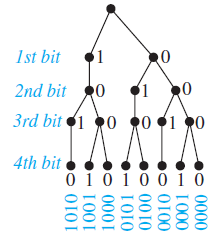
\includegraphics{images/exemplo21.png}
\caption{Bit Strings of Length Four without Consecutive 1s.}
\label{fig:ex21}
\end{figure}

%example 22
\item A playoff between two teams consists of at most five games.
The first team that wins three games wins the playoff.
In how many different ways can the playoff occur?

Solution: The tree diagram in Figure~\ref{fig:ex22} displays all the ways the playoff can proceed, with the winner of each game shown.
We see that there are 20 different ways for the playoff to occur.

\begin{figure}[h]
\centering
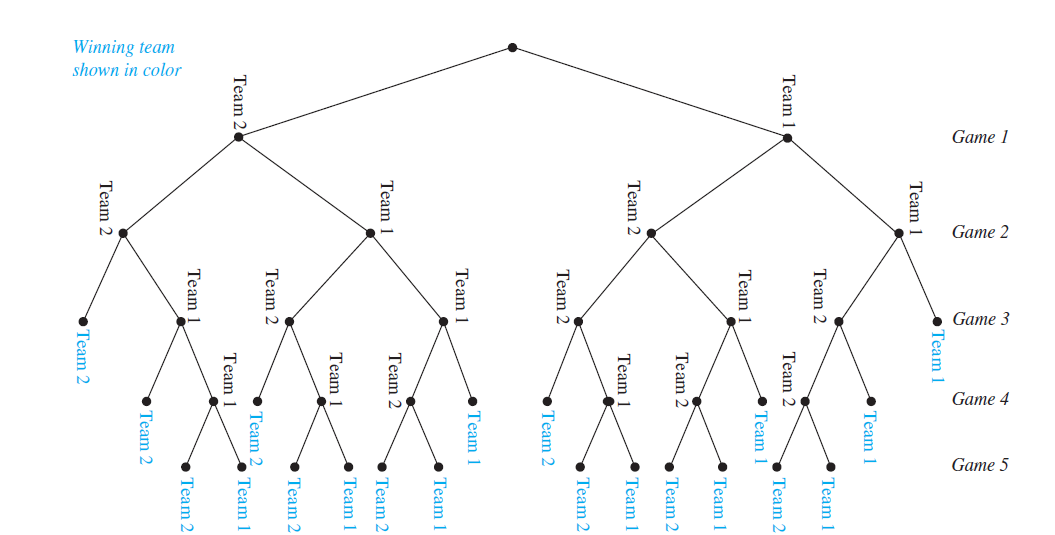
\includegraphics[height=6cm,width=1.2\textwidth]{images/exemplo22.png}
\caption{Best Three Games Out of Five Playoffs.}
\label{fig:ex22}
\end{figure}

%example 23
\item Suppose that “I Love New Jersey” T-shirts come in five different sizes: S, M, L, XL, and XXL.
Further suppose that each size comes in four colors, white, red, green, and black, except for XL, which comes only in red, green, and black, and XXL, which comes only in green and black.
How many different shirts does a souvenir shop have to stock to have at least one of each available size and color of the T-shirt?

Solution: The tree diagram in Figure~\ref{fig:ex23} displays all possible size and color pairs.
It follows that the souvenir shop owner needs to stock 17 different T-shirts.

\begin{figure}[h]
\centering
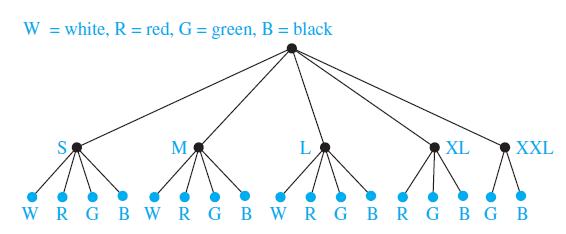
\includegraphics{images/exemplo23.png}
\caption{Counting Varieties of T-Shirts.}
\label{fig:ex23}
\end{figure}

\end{enumerate}

Exercises
\begin{enumerate}
%exercise 1
\item There are 18 mathematics majors and 325 computer science majors at a college.
 \begin{enumerate}[label=(\alph*)]
 \item  In how many ways can two representatives be picked so that one is a mathematics major and the other is a computer science major?
 \item  In how many ways can one representative be picked who is either a mathematics major or a computer science major?
 \end{enumerate}
%exercise 2
\item An office building contains 27 floors and has 37 offices on each floor. 
How many offices are in the building?
%exercise 3
\item A multiple-choice test contains 10 questions.
There are four possible answers for each question.
\begin{enumerate}[label=(\alph*)]
\item In how many ways can a student answer the questions on the test if the student answers every question?
\item In how many ways can a student answer the questions on the test if the student can leave answers blank?
\end{enumerate}
%exercise 4
\item A particular brand of shirt comes in 12 colors, has a male version and a female version, and comes in three sizes for each sex.
How many different types of this shirt are made?
%exercise 5
\item Six different airlines fly from New York to Denver and seven fly from Denver to San Francisco.
How many different pairs of airlines can you choose on which to book a trip from NewYork to San Francisco via Denver, when you pick an airline for the flight to Denver and an airline for the continuation flight to San Francisco?
%exercise 6
\item There are four major auto routes from Boston to Detroit and six from Detroit to Los Angeles.
How many major auto routes are there from Boston to Los Angeles via Detroit?
%exercise 7
\item How many different three-letter initials can people have?
%exercise 8
\item How many different three-letter initials with none of the letters repeated can people have?
%exercise 9
\item How many different three-letter initials are there that begin with an A?
%exercise 10
\item How many bit strings are there of length eight?
%exercise 11
\item How many bit strings of length ten both begin and end with a 1?
%exercise 12
\item How many bit strings are there of length six or less, not counting the empty string?
%exercise 13
\item How many bit strings with length not exceeding n, where n is a positive integer, consist entirely of 1s, not counting the empty string?
%exercise 14
\item How many bit strings of length n, where n is a positive integer, start and end with 1s?
%exercise 15
\item How many strings are there of lowercase letters of length four or less, not counting the empty string?
%exercise 16
\item How many strings are there of four lowercase letters that have the letter x in them?
%exercise 17
\item How many strings of five ASCII characters contain the character @ (“at” sign) at least once? [Note: There are 128 different ASCII characters.]
%exercise 18
\item How many 5-element DNA sequences
\begin{enumerate}[label=(\alph*)]
\item end with A?
\item start with T and end with G?
\item contain only A and T?
\item do not contain C?
\end{enumerate}
%exercise 19
\item How many 6-element RNA sequences
\begin{enumerate}[label=(\alph*)]
\item do not contain U?
\item end with GU?
\item start with C?
\item contain only A or U?
\end{enumerate}
%exercise 20
\item How many positive integers between 5 and 31
\begin{enumerate}[label=(\alph*)]
\item are divisible by 3? Which integers are these?
\item are divisible by 4? Which integers are these?
\item are divisible by 3 and by 4? Which integers are these?
\end{enumerate}
%exercise 21
\item How many positive integers between 50 and 100
\begin{enumerate}[label=(\alph*)]
\item are divisible by 7? Which integers are these?
\item are divisible by 11? Which integers are these?
\item are divisible by both 7 and 11? Which integers are
these?
\end{enumerate}
%exercise 22
\item How many positive integers less than 1000
\begin{enumerate}[label=(\alph*)]
\item are divisible by 7?
\item are divisible by 7 but not by 11?
\item are divisible by both 7 and 11?
\item are divisible by either 7 or 11?
\item are divisible by exactly one of 7 and 11?
\item are divisible by neither 7 nor 11?
\item have distinct digits?
\item have distinct digits and are even?
\end{enumerate}
%exercise 23
\item How many positive integers between 100 and 999 inclusive
\begin{enumerate}[label=(\alph*)]
\item are divisible by 7?
\item are odd?
\item have the same three decimal digits?
\item are not divisible by 4?
\item are divisible by 3 or 4?
\item are not divisible by either 3 or 4?
\item are divisible by 3 but not by 4?
\item are divisible by 3 and 4?
\end{enumerate}
%exercise 24
\item How many positive integers between 1000 and 9999 inclusive 
\begin{enumerate}[label=(\alph*)]
\item are divisible by 9?
\item are even?
\item have distinct digits?
\item are not divisible by 3?
\item are divisible by 5 or 7?
\item are not divisible by either 5 or 7?
\item are divisible by 5 but not by 7?
\item are divisible by 5 and 7?
\end{enumerate}
%exercise 25
\item How many strings of three decimal digits
\begin{enumerate}[label=(\alph*)]
\item do not contain the same digit three times?
\item begin with an odd digit?
\item have exactly two digits that are 4s?
\end{enumerate}
%exercise 26
\item How many strings of four decimal digits
\begin{enumerate}[label=(\alph*)]
\item do not contain the same digit twice?
\item end with an even digit?
\item have exactly three digits that are 9s?
\end{enumerate}
%exercise 27
\item A committee is formed consisting of one representative from each of the 50 states in the United States, where the representative from a state is either the governor or one of the two senators from that state.
How many ways are there to form this committee?
%exercise 28
\item How many license plates can be made using either three digits followed by three uppercase English letters or three uppercase English letters followed by three digits?
%exercise 29
\item How many license plates can be made using either two uppercase English letters followed by four digits or two digits followed by four uppercase English letters?
%exercise 30
\item How many license plates can be made using either three uppercase English letters followed by three digits or four uppercase English letters followed by two digits?
%exercise 31
\item How many license plates can be made using either two or three uppercase English letters followed by either two or three digits?
%exercise 32
\item How many strings of eight uppercase English letters are there
\begin{enumerate}[label=(\alph*)]
\item if letters can be repeated?
\item if no letter can be repeated?
\item that start with X, if letters can be repeated?
\item that start with X, if no letter can be repeated?
\item that start and end with X, if letters can be repeated?
\item that start with the letters BO (in that order), if letters can be repeated?
\item that start and end with the letters BO (in that order), if letters can be repeated?
\item that start or end with the letters BO (in that order), if letters can be repeated?
\end{enumerate}
%exercise 33
\item How many strings of eight English letters are there
\begin{enumerate}[label=(\alph*)]
\item that contain no vowels, if letters can be repeated?
\item that contain no vowels, if letters cannot be repeated?
\item that start with a vowel, if letters can be repeated?
\item that start with a vowel, if letters cannot be repeated?
\item that contain at least one vowel, if letters can be repeated?
\item that contain exactly one vowel, if letters can be repeated?
\item that start with X and contain at least one vowel, if letters can be repeated?
\item that start and end with X and contain at least one vowel, if letters can be repeated?
\end{enumerate}
%exercise 34
\item How many different functions are there from a set with 10 elements to sets with the following numbers of elements?
\begin{enumerate}
\item 2  \inlineitem 3  \inlineitem 4  \inlineitem 5
\end{enumerate}
%exercise 35 
\item How many one-to-one functions are there from a set with five elements to sets with the following number of elements?
\begin{enumerate}
\item 4 \inlineitem 5 \inlineitem 6 \inlineitem 7
\end{enumerate}
%exercise 36
\item How many functions are there from the set {1, 2, . . . , n}, where n is a positive integer, to the set {0, 1}?
%exercise 37
\item How many functions are there from the set {1, 2, . . . , n}, where n is a positive integer, to the set {0, 1}
\begin{enumerate}[label=(\alph*)]
\item that are one-to-one?
\item that assign 0 to both 1 and n?
\item that assign 1 to exactly one of the positive integers less than n?
\end{enumerate}
%exercise 38
\item How many partial functions (see Section 2.3) are there from a set with five elements to sets with each of these number of elements?
\begin{enumerate}
\item 1 \inlineitem 2 \inlineitem 5 \inlineitem 9
\end{enumerate}
%exercise 39
\item How many partial functions are there from a set with m elements to a set with n elements, where m and n are positive integers?
%exercise 40
\item How many subsets of a set with 100 elements have more than one element?
%exercise 41
\item Apalindrome is a string whose reversal is identical to the string. How many bit strings of length n are palindromes?
%exercise 42
\item How many 4-element DNA sequences
\begin{enumerate}
\item do not contain the base T?
\item contain the sequence ACG?
\item contain all four bases A, T, C, and G?
\item contain exactly three of the four bases A, T, C, and G?
\end{enumerate}
%exercise 43
\item How many 4-element RNA sequences
\begin{enumerate}
\item contain the base U?
\item do not contain the sequence CUG?
\item do not contain all four bases A, U, C, and G?
\item contain exactly two of the four bases A, U, C, and G?
\end{enumerate}
%exercise 44
\item How many ways are there to seat four of a group of ten people around a circular table where two seatings are considered the same when everyone has the same immediate left and immediate right neighbor?
%exercise 45
\item. How many ways are there to seat six people around a circular table where two seatings are considered the same when everyone has the same two neighbors without regard to whether they are right or left neighbors?
%exercise 46
\item In how many ways can a photographer at a wedding arrange 6 people in a row from a group of 10 people, where the bride and the groom are among these 10 people, if
\begin{enumerate}[label=(\alph*)]
\item the bride must be in the picture?
\item both the bride and groom must be in the picture?
\item exactly one of the bride and the groom is in the picture?
\end{enumerate}
%exercise 47
\item In how many ways can a photographer at a wedding arrange six people in a row, including the bride and groom, if
\begin{enumerate}[label=(\alph*)]
\item the bride must be next to the groom?
\item the bride is not next to the groom?
\item the bride is positioned somewhere to the left of the
groom?
\end{enumerate}
%exercise 47
\item How many bit strings of length seven either begin with two 0s or end with three 1s?
%exercise 49
\item How many bit strings of length 10 either begin with three 0s or end with two 0s?
%exercise 50
\onestaritem How many bit strings of length 10 contain either five consecutive 0s or five consecutive 1s?
%exercise 51
\twostaritem How many bit strings of length eight contain either three consecutive 0s or four consecutive 1s?
%exercise 52
\item Every student in a discrete mathematics class is either a computer science or a mathematics major or is a joint major in these two subjects. How many students are in the class if there are 38 computer science majors (including joint majors), 23 mathematics majors (including joint majors), and 7 joint majors?
%exercise 53
\item How many positive integers not exceeding 100 are divisible either by 4 or by 6?
%exercise 54
\item How many different initials can someone have if a person has at least two, but no more than five, different initials?
Assume that each initial is one of the 26 uppercase letters of the English language.
%exercise 55
\item Suppose that a password for a computer system must have at least 8, but no more than 12, characters, where each character in the password is a lowercase English letter, an uppercase English letter, a digit, or one of the six special characters \emph{*, >, <, !, +,} and \emph{=}.
\begin{enumerate}
\item How many different passwords are available for this computer system?
\item How many of these passwords contain at least one occurrence of at least one of the six special characters?
\item Using your answer to part (a), determine how long it takes a hacker to try every possible password, assuming that it takes one nanosecond for a hacker to check each possible password.
\end{enumerate}
%exercise 56
\item The name of a variable in the C programming language is a string that can contain uppercase letters, lowercase letters, digits, or underscores. Further, the first character in the string must be a letter, either uppercase or lowercase, or an underscore.
If the name of a variable is determined by its first eight characters, how many different variables can be named in C? (Note that the name of a variable may contain fewer than eight characters.)
%exercise 57
\item The name of a variable in the JAVA programming language is a string of between 1 and 65,535 characters, inclusive, where each character can be an uppercase or a lowercase letter, a dollar sign, an underscore, or a digit, except that the first character must not be a digit.
Determine the number of different variable names in JAVA.
%exercise 58
\item The International Telecommunications Union (ITU) specifies that a telephone number must consist of a country code with between 1 and 3 digits, except that the code 0 is not available for use as a country code, followed by a number with at most 15 digits.
How many available possible telephone numbers are there that satisfy these restrictions?
%exercise 59
\item Suppose that at some future time every telephone in the world is assigned a number that contains a country code 1 to 3 digits long, that is, of the form X, XX, or XXX, followed by a 10-digit telephone number of the form NXX-NXX-XXXX (as described in Example 8).
How many different telephone numbers would be available worldwide under this numbering plan?
%exercise 60
\item A key in the Vigenère cryptosystem is a string of English letters, where the case of the letters does not matter.
How many different keys for this cryptosystem are there with three, four, five, or six letters?
%exercise 61
\item A wired equivalent privacy (WEP) key for a wireless fidelity (WiFi) network is a string of either 10, 26, or 58 hexadecimal digits.
How many different WEP keys are there?
%exercise 62
\item Suppose that \emph{p} and \emph{q} are prime numbers and that \emph{n = pq}.
Use the principle of inclusion–exclusion to find the number of positive integers not exceeding n that are relatively prime to n.
%exercise 63
\item Use the principle of inclusion–exclusion to find the number of positive integers less than 1,000,000 that are not divisible by either 4 or by 6.
%exercise 64
\item Use a tree diagram to find the number of bit strings of length four with no three consecutive 0s.
%exercise 65
\item How many ways are there to arrange the letters a, b, c, and d such that a is not followed immediately by b?
%exercise 66
\item Use a tree diagram to find the number of ways that the World Series can occur, where the first team that wins four games out of seven wins the series.
%exercise 67
\item Use a tree diagram to determine the number of subsets of {3, 7, 9, 11, 24} with the property that the sum of the elements in the subset is less than 28.
%exercise 68
\item \begin{enumerate}[label=(\alph*)]
\item Suppose that a store sells six varieties of soft drinks: cola, ginger ale, orange, root beer, lemonade, and cream soda.
Use a tree diagram to determine the number of different types of bottles the store must stock to have all varieties available in all size bottles if all varieties are available in 12-ounce bottles, all but lemonade are available in 20-ounce bottles, only cola and ginger ale are available in 32-ounce bottles, and all but lemonade and cream soda are available in 64-ounce bottles?
\item Answer the question in part (a) using counting rules.
\end{enumerate} 
%exercise 69
\item \begin{enumerate}
\item Suppose that a popular style of running shoe is available for both men and women.
The woman's shoe comes in sizes 6, 7, 8, and 9, and the man's shoe comes in sizes 8, 9, 10, 11, and 12.
The man's shoe comes in white and black, while the woman's shoe comes in white, red, and black.
Use a tree diagram to determine the number of different shoes that a store has to stock to have at least one pair of this type of running shoe for all available sizes and colors for both men and women.
\item Answer the question in part (a) using counting rules.
\end{enumerate}
%exercise 70 
\onestaritem Use the product rule to show that there are $2^{2^{n}}$ different truth tables for propositions in n variables.
%exercise 71
\item Use mathematical induction to prove the sum rule for m tasks from the sum rule for two tasks.
%exercise 72
\item Use mathematical induction to prove the product rule for m tasks from the product rule for two tasks.
%exercise 73
\item How many diagonals does a convex polygon with n sides have? (Recall that a polygon is convex if every line segment connecting two points in the interior or boundary of the polygon lies entirely within this set and that a diagonal of a polygon is a line segment connecting two vertices that are not adjacent.)
%exercise 74
\item Data are transmitted over the Internet in \textbf{datagrams}, which are structured blocks of bits.
Each datagram contains header information organized into a maximum of 14 different fields (specifying many things, including the source and destination addresses) and a data area that contains the actual data that are transmitted.
One of the 14 header fields is the \textbf{header length field} (denoted by HLEN), which is specified by the protocol to be 4 bits long and that specifies the header length in terms of 32-bit blocks of bits.
For example, if HLEN = 0110, the header is made up of six 32-bit blocks.
Another of the 14 header fields is the 16-bit-long \textbf{total length field} (denoted by TOTAL LENGTH), which specifies the length in bits of the entire datagram, including both the header fields and the data area.
The length of the data area is the total length of the datagram minus the length of the header.
\begin{enumerate}[label=(\alph*)]
\item The largest possible value of TOTAL LENGTH (which is 16 bits long) determines the maximum total length in octets (blocks of 8 bits) of an Internet datagram.
What is this value?
\item The largest possible value of HLEN (which is 4 bits long) determines the maximum total header length in 32-bit blocks.
What is this value?
What is the maximum total header length in octets?
\item The minimum (and most common) header length is 20 octets.
What is the maximum total length in octets of the data area of an Internet datagram?
\item How many different strings of octets in the data area can be transmitted if the header length is 20 octets and the total length is as long as possible?
\end{enumerate}
\end{enumerate}

\section{The Pigeonhole Principle}
\begin{enumerate}[label=Example~\arabic*]
%example 1
\item Among any group of 367 people, there must be at least two with the same birthday, because there are only 366 possible birthdays.
%example 2
\item In any group of 27 English words, there must be at least two that begin with the same letter, because there are 26 letters in the English alphabet.
%example 3
\item How many students must be in a class to guarantee that at least two students receive the same score on the final exam, if the exam is graded on a scale from 0 to 100 points?

Solution: There are 101 possible scores on the final.
The pigeonhole principle shows that among any 102 students there must be at least 2 students with the same score.

%example 4
\item Show that for every integer \emph{n} there is a multiple of \emph{n} that has only 0s and 1s in its decimal expansion.

Solution: Let n be a positive integer.
Consider the \emph{n + 1} integers 1, 11, 111, . . . , 11 . . . 1 (where the last integer in this list is the integer with \emph{n + 1 1s} in its decimal expansion).
Note that there are \emph{n} possible remainders when an integer is divided by \emph{n}.
Because there are \emph{n + 1} integers in this list, by the pigeonhole principle there must be two with the same remainder when divided by \emph{n}.
The larger of these integers less the smaller one is a multiple of \emph{n}, which has a decimal expansion consisting entirely of 0s and 1s.

%example 5
\item Among 100 people there are at least $\lceil 100/12 \rceil$ = 9 who were born in the same month.

%example6
What is the minimum number of students required in a discrete mathematics class to be sure that at least six will receive the same grade, if there are five possible grades, A, B, C, D, and F?

Solution: The minimum number of students needed to ensure that at least six students receive the same grade is the smallest integer N such that $\lceil N/5 \rceil$ = 6.
The smallest such integer is $N = 5 \cdot 5 + 1 = 26$.
If you have only 25 students, it is possible for there to be five who have received each grade so that no six students have received the same grade.
Thus, 26 is the minimum number of students needed to ensure that at least six students will receive the same grade.

%example 7
\item \begin{enumerate}[label=(\alph*)]
\item How many cards must be selected from a standard deck of 52 cards to guarantee that at least three cards of the same suit are chosen?
\item How many must be selected to guarantee that at least three hearts are selected?
\end{enumerate}

Solution: \begin{enumerate}[label=(\alph*)]
\item Suppose there are four boxes, one for each suit, and as cards are selected they are placed in the box reserved for cards of that suit.
Using the generalized pigeonhole principle, we see that if N cards are selected, there is at least one box containing at least $\lceil N/4\rceil$ cards.
Consequently, we know that at least three cards of one suit are selected if $\lceil N/4\rceil \geq 3$.
The smallest integer N such that $\lceil N/4\rceil \geq 3$ is $N = 2 \cdot 4 + 1 = 9$, so nine cards suffice.
Note that if eight cards are selected, it is possible to have two cards of each suit, so more than eight cards are needed.
Consequently, nine cards must be selected to guarantee that at least three cards of one suit are chosen.
One good way to think about this is to note that after the eighth card is chosen, there is no way to avoid having a third card of some suit.
\item We do not use the generalized pigeonhole principle to answer this question, because we want to make sure that there are three hearts, not just three cards of one suit.
Note that in the worst case, we can select all the clubs, diamonds, and spades, 39 cards in all, before we select a single heart.
The next three cards will be all hearts, so we may need to select 42 cards to get three hearts.
\end{enumerate}

%example 8
\item What is the least number of area codes needed to guarantee that the 25 million phones in a state can be assigned distinct 10-digit telephone numbers? (Assume that telephone numbers are of the form \emph{NXX-NXX-XXXX}, where the first three digits form the area code, N represents a digit from 2 to 9 inclusive, and X represents any digit.)

Solution: There are eight million different phone numbers of the form \emph{NXX-XXXX} (as shown in Example 8 of Section 6.1).
Hence, by the generalized pigeonhole principle, among 25 million telephones, at least $\lceil 25,000,000/8,000,000\rceil = 4$ of them must have identical phone numbers.
Hence, at least four area codes are required to ensure that all 10-digit numbers are different. 

%example 9
\item Suppose that a computer science laboratory has 15 workstations and 10 servers.
A cable can be used to directly connect a workstation to a server.
For each server, only one direct connection to that server can be active at any time.
We want to guarantee that at any time any set of 10 or fewer workstations can simultaneously access different servers via direct connections.
Although we could do this by connecting every workstation directly to every server (using 150 connections), what is the minimum number of direct connections needed to achieve this goal?

Solution: Suppose that we label the workstations \emph{$W_1,W_2, ~\cdot~\cdot~\cdot , W_{15}$} and the servers \emph{$S_1, S_2, \cdot~\cdot~\cdot , S_{10}$}.
Furthermore, suppose that we connect $W_k$ to $S_k$ for \emph{$k = 1, 2,~\cdot~\cdot~\cdot , 10$} and each of $W_{11},W_{12},W_{13},W_{14}$, and $W_{15}$ to all 10 servers.
We have a total of 60 direct connections.
Clearly any set of 10 or fewer workstations can simultaneously access different servers.
We see this by noting that if workstation $W_j$ is included with $1 \leq j \leq 10$, it can access server $S_j$, and for each workstation $W_k$ with $k \geq 11$ included, there must be a corresponding workstation $W_j$ with $1 \leq j \leq 10$ not included, so $W_k$ can access server $S_j$ . (This follows because there are at least as many available servers Sj as there are workstations $W_j$ with $1 \leq j \leq 10$ not included.)
Now suppose there are fewer than 60 direct connections between workstations and servers.
Then some server would be connected to at most $\lfloor 59/10\rfloor = 5$ workstations. (If all servers were connected to at least six workstations, there would be at least $6 \cdot 10 = 60$ direct connections.)
This means that the remaining nine servers are not enough to allow the other 10 workstations to simultaneously access different servers.
Consequently, at least 60 direct connections are needed.
It follows that 60 is the answer.

%example 10
\item During a month with 30 days, a baseball team plays at least one game a day, but no more than 45 games. 
Show that there must be a period of some number of consecutive days during which the team must play exactly 14 games.

Solution: Let $a_j$ be the number of games played on or before the \emph{j th} day of the month.
Then $a_1, a_2,~\cdot~\cdot~\cdot, a_{30}$ is an increasing sequence of distinct positive integers, with $1 \leq a_j \leq 45$.
Moreover, $a_1 + 14, a_2 + 14,~\cdot~\cdot~\cdot, a_{30} + 14$ is also an increasing sequence of distinct positive integers, with $15 \leq a_j + 14 \leq 59$.
The 60 positive integers $a_1, a_2,~\cdot~\cdot~\cdot, a_{30}, a_1 + 14, a_2 + 14,~\cdot~\cdot~\cdot, a_{30} + 14$ are all less than or equal to 59.
Hence, by the pigeonhole principle two of these integers are equal.
Because the integers $a_j , j = 1, 2,~\cdot~\cdot~\cdot, 30$ are all distinct and the integers $a_j + 14, j = 1, 2,~\cdot~\cdot~\cdot, 30$ are all distinct, there must be indices \emph{i} and \emph{j} with $a_i = a_j + 14$.
This means that exactly 14 games were played from day \emph{j + 1} to day \emph{i}.

%example 11
\item Show that among any \emph{n + 1} positive integers not exceeding \emph{2n} there must be an integer that divides one of the other integers.

Solution: Write each of the \emph{n + 1} integers $a_1, a_2,~\cdot~\cdot~\cdot, a_{n+1}$ as a power of 2 times an odd integer.
In other words, let $a_j = 2^{k_j}q_j$ for $j = 1, 2,~\cdot~\cdot~\cdot, n + 1$, where $k_j$ is a nonnegative integer and $q_j$ is odd.
The integers $q_1, q_2,~\cdot~\cdot~\cdot, q_{n+1}$ are all odd positive integers less than \emph{2n}.
Because there are only \emph{n} odd positive integers less than \emph{2n}, it follows from the pigeonhole principle that two of the integers $q_1, q_2,~\cdot~\cdot~\cdot, q_{n+1}$ must be equal.
Therefore, there are distinct integers \emph{i} and \emph{j} such that $q_i = q_j$.
Let \emph{q }be the common value of $q_i$ and $q_j$.
Then, $a_i = 2^{k_i}q$ and $a_j = 2^{k_j}q$.
It follows that if $k_i < k_j$ , then $a_i$ divides $a_j$; while if $k_i > k_j$ , then $a_j$ divides $a_i$.

%example 12
\item The sequence 8, 11, 9, 1, 4, 6, 12, 10, 5, 7 contains 10 terms.
Note that $10 = 3^{2} + 1$.
There are four strictly increasing subsequences of length four, namely, 1, 4, 6, 12; 1, 4, 6, 7;
1, 4, 6, 10; and 1, 4, 5, 7. There is also a strictly decreasing subsequence of length four, namely, 11, 9, 6, 5.

%example 13
\item Assume that in a group of six people, each pair of individuals consists of two friends or two enemies.
Show that there are either three mutual friends or three mutual enemies in the group.

Solution: Let A be one of the six people.
Of the five other people in the group, there are either three or more who are friends of A, or three or more who are enemies of A.
This follows from the generalized pigeonhole principle, because when five objects are divided into two sets, one of the sets has at least $\lceil 5/2\rceil = 3$ elements.
In the former case, suppose that B, C, and D are friends of A.
If any two of these three individuals are friends, then these two and A form a group of three mutual friends.
Otherwise, B, C, and D form a set of three mutual enemies.
The proof in the latter case, when there are three or more enemies of A, proceeds in a similar manner.

\end{enumerate}
Exercises
%exercises
\begin{enumerate}
%exercise 1
\item Show that in any set of six classes, each meeting regularly once a week on a particular day of the week, there must be two that meet on the same day, assuming that no classes are held on weekends.
%exercise 2
\item Show that if there are 30 students in a class, then at least two have last names that begin with the same letter.
%exercise 3
\item A drawer contains a dozen brown socks and a dozen black socks, all unmatched.
A man takes socks out at random in the dark.
\begin{enumerate}[label=(\alph*)]
\item How many socks must he take out to be sure that he has at least two socks of the same color?
\item How many socks must he take out to be sure that he has at least two black socks?
\end{enumerate}
%exercise 4
\item A bowl contains 10 red balls and 10 blue balls.
A woman selects balls at random without looking at them.
\begin{enumerate}[label=(\alph*)]
\item How many balls must she select to be sure of having at least three balls of the same color?
\item How many balls must she select to be sure of having at least three blue balls?
\end{enumerate}
%exercise 5
\item Show that among any group of five (not necessarily consecutive) integers, there are two with the same remainder when divided by 4.
%exercise 6
\item Let d be a positive integer.
Show that among any group of \emph{d + 1} (not necessarily consecutive) integers there are two with exactly the same remainder when they are divided by \emph{d}.
%exercise 7
\item Let n be a positive integer.
Show that in any set of \emph{n} consecutive integers there is exactly one divisible by \emph{n}.
%exercise 8
\item Show that if f is a function from S to T , where S and T are finite sets with |S| > |T|, then there are elements $s_1$ and $s_2$ in S such that $f(_s1) = f(s_2)$, or in other words, f is not one-to-one.
%exercise 9
\item What is the minimum number of students, each of whom comes from one of the 50 states, who must be enrolled in a university to guarantee that there are at least 100 who come from the same state?
%exercise 10
\onestaritem Let $(x_i, y_i )$, i = 1, 2, 3, 4, 5, be a set of five distinct points with integer coordinates in the xy plane.
Show that the midpoint of the line joining at least one pair of these points has integer coordinates.
%exercise 11
\onestaritem Let $(x_i, y_i, z_i )$, i = 1, 2, 3, 4, 5, 6, 7, 8, 9, be a set of nine distinct points with integer coordinates in xyz space.
Show that the midpoint of at least one pair of these points has integer coordinates.
%exercise 12
\item How many ordered pairs of integers (a, b) are needed to guarantee that there are two ordered pairs $(a_1, b_1)$ and $(a_2, b_2)$ such that $a_1 mod 5 = a_2 mod 5$ and $b_1 mod 5 = b_2 mod 5$?
%exercise 13
\item \begin{enumerate}[label=(\alph*)]
\item Show that if five integers are selected from the first eight positive integers, there must be a pair of these integers with a sum equal to 9.
\item Is the conclusion in part (a) true if four integers are selected rather than five?
\end{enumerate}
%exercise 14
\item \begin{enumerate}[label=(\alph*)]
\item Show that if seven integers are selected from the first 10 positive integers, there must be at least two pairs of these integers with the sum 11.
\item Is the conclusion in part (a) true if six integers are selected rather than seven?
\end{enumerate}
%exercise 15
\item How many numbers must be selected from the set {1, 2, 3, 4, 5, 6} to guarantee that at least one pair of these numbers add up to 7?
%exercise 16
\item How many numbers must be selected from the set {1, 3, 5, 7, 9, 11, 13, 15} to guarantee that at least one pair of these numbers add up to 16?
%exercise 17
\item A company stores products in a warehouse.
Storage bins in this warehouse are specified by their aisle, location in the aisle, and shelf.
There are 50 aisles, 85 horizontal locations in each aisle, and 5 shelves throughout the warehouse.
What is the least number of products the company can have so that at least two products must be stored in the same bin?
%exercise 18
\item Suppose that there are nine students in a discrete mathematics class at a small college.
\begin{enumerate}[label=(\alph*)]
\item Show that the class must have at least five male students or at least five female students.
\item Show that the class must have at least three male students or at least seven female students.
\end{enumerate}
%exercise 19
\item Suppose that every student in a discrete mathematics class of 25 students is a freshman, a sophomore, or a junior.
\begin{enumerate}[label=(\alph*)]
\item Show that there are at least nine freshmen, at least nine sophomores, or at least nine juniors in the class.
\item Show that there are either at least three freshmen, at least 19 sophomores, or at least five juniors in the class.
\end{enumerate}
%exercise 20
\item Find an increasing subsequence of maximal length and a decreasing subsequence of maximal length in the sequence 22, 5, 7, 2, 23, 10, 15, 21, 3, 17.
%exercise 21
\item Construct a sequence of 16 positive integers that has no increasing or decreasing subsequence of five terms.
%exercise 22
\item Show that if there are 101 people of different heights standing in a line, it is possible to find 11 people in the order they are standing in the line with heights that are either increasing or decreasing.
%exercise 23
\onestaritem Show that whenever 25 girls and 25 boys are seated around a circular table there is always a person both of whose neighbors are boys.
%exercise 24
\twostaritem Suppose that 21 girls and 21 boys enter a mathematics competition.
Furthermore, suppose that each entrant solves at most six questions, and for every boy-girl pair, there is at least one question that they both solved.
Show that there is a question that was solved by at least three girls and at least three boys.
%exercise 25
\onestaritem Describe an algorithm in pseudocode for producing the largest increasing or decreasing subsequence of a sequence of distinct integers.
%exercise 26
\item Show that in a group of five people (where any two people are either friends or enemies), there are not necessarily three mutual friends or three mutual enemies.
%exercise 27
\item Show that in a group of 10 people (where any two people are either friends or enemies), there are either three mutual friends or four mutual enemies, and there are either three mutual enemies or four mutual friends.
%exercise 28
\item Use Exercise 27 to show that among any group of 20 people (where any two people are either friends or enemies), there are either four mutual friends or four mutual enemies.
%exercise 29
\item Show that if \emph{n} is an integer with $n \geq 2$, then the Ramsey number \emph{R(2, n)} equals n.
%exercise 30
\item Show that if \emph{m} and \emph{n} are integers with $m \geq 2$ and $n \geq 2$, then the Ramsey numbers \emph{R(m, n)} and \emph{R(n, m)} are equal.
%exercise 31]
\item Show that there are at least six people in California (population: 37 million) with the same three initials who were born on the same day of the year (but not necessarily in the same year).
Assume that everyone has three initials.
%exercise 32
\item Show that if there are 100,000,000 wage earners in the United States who earn less than 1,000,000 dollars (but at least a penny), then there are two who earned exactly the same amount of money, to the penny, last year.
%exercise 33
\item In the \emph{17th} century, there were more than 800,000 inhabitants of Paris.
At the time, it was believed that no one had more than 200,000 hairs on their head.
Assuming these numbers are correct and that everyone has at least one hair on their head (that is, no one is completely bald), use the pigeonhole principle to show, as the French writer Pierre Nicole did, that there had to be two Parisians with the same number of hairs on their heads.
Then use the generalized pigeonhole principle to show that there had to be at least five Parisians at that time with the same number of hairs on their heads.
%exercise 34
\item Assuming that no one has more than 1,000,000 hairs on the head of any person and that the population of New York City was 8,008,278 in 2010, show there had to be at least nine people in NewYork City in 2010 with the same number of hairs on their heads.
%exercise 35
\item There are 38 different time periods during which classes at a university can be scheduled.
If there are 677 different classes, how many different rooms will be needed?
%exercise 36
\item A computer network consists of six computers.
Each computer is directly connected to at least one of the other computers.
Show that there are at least two computers in the network that are directly connected to the same number of other computers.
%exercise 37
\item A computer network consists of six computers.
Each computer is directly connected to zero or more of the other computers.
Show that there are at least two computers in the network that are directly connected to the same number of other computers. [\textit{Hint}: It is impossible to have a computer linked to none of the others and a computer linked to all the others.]
%exercise 38
\item Find the least number of cables required to connect eight computers to four printers to guarantee that for every choice of four of the eight computers, these four computers can directly access four different printers.
Justify your answer.
%exercise 39
\item Find the least number of cables required to connect 100 computers to 20 printers to guarantee that 2every subset of 20 computers can directly access 20 different printers. (Here, the assumptions about cables and computers are the same as in Example 9.)
Justify your answer.
%exercise 40
\onestaritem Prove that at a party where there are at least two people, there are two people who know the same number of other people there.
%exercise 41
\item An arm wrestler is the champion for a period of 75 hours. (Here, by an hour, we mean a period starting from an exact hour, such as 1 p.m., until the next hour.)
The arm wrestler had at least one match an hour, but no more than 125 total matches.
Show that there is a period of consecutive hours during which the arm wrestler had exactly 24 matches.
%exercise 42
\onestaritem Is the statement in Exercise 41 true if 24 is replaced by 
\begin{enumerate}[label=(\alph*)]
\item 2? \inlineitem 23? \inlineitem 25? \inlineitem 30?
\end{enumerate}
%exercise 43
\item Show that if \textit{f} is a function from \emph{S} to \emph{T} , where \emph{S} and \emph{T} are nonempty finite sets and $m = \lceil |S| / |T |\rceil$, then there are at least \emph{m} elements of \emph{S} mapped to the same value of \emph{T}.
That is, show that there are distinct elements $s_1, s_2,~\cdot~\cdot~\cdot, s_m$ of \emph{S} such that $\textit{f}(s_1) = \textit{f}(s_2) =~\cdot~\cdot~\cdot= \textit{f}(s_m)$.
%exercise 44
\item There are 51 houses on a street.
Each house has an address between 1000 and 1099, inclusive.
Show that at least two houses have addresses that are consecutive integers.
%exercise 45
\onestaritem Let \emph{x} be an irrational number.
Show that for some positive integer \emph{j} not exceeding the positive integer \emph{n}, the absolute value of the difference between $j_x$ and the nearest integer to $j_x$ is less than 1/n.
%exercise 46
\item Let $n_1, n_2,~\cdot~\cdot~\cdot, n_t$ be positive integers.
Show that if $n_1, n_2,~\cdot~\cdot~\cdot, n_t - t + 1$ objects are placed into \emph{t} boxes, then for some \emph{i}, $i = 1, 2,~\cdot~\cdot~\cdot, t$, the \emph{ith} box contains at least $n_i$ objects.
%exercise 47
\onestaritem An alternative proof of Theorem 3 based on the generalized pigeonhole principle is outlined in this exercise.
The notation used is the same as that used in the proof in the text.
\begin{enumerate}[label=(\alph*)]
\item Assume that $i_k \leq n$ for $k = 1, 2, . . . , n^{2} + 1$.
Use the generalized pigeonhole principle to show that there are n + 1 terms $a_{k_1}, a_{k_2},~\cdot~\cdot~\cdot, a_{k_{n+1}}$ with $i_{k_1} = i_{k_2} = ~\cdot~\cdot~\cdot = i_{k_{n+1}}$ , where $1 \leq k_1 < k_2 <~\cdot~\cdot~\cdot< k_{n+1}$.
\item Show that $a_{k_j} > a_{k_{j+1}}$ for $j = 1, 2,~\cdot~\cdot~\cdot, n$. [\textit{Hint}: Assume that $a_{k_j} < a_{k_{j+1}}$ , and show that this implies that $i_{k_j} > i_{k_{j+1}}$ , which is a contradiction.]
\item Use parts (a) and (b) to sho wthat if there is no increasing subsequence of length \emph{n + 1}, then there must be a decreasing subsequence of this length.
\end{enumerate}
\end{enumerate}

\section{Permutations and Combinations}
\begin{enumerate}[label=Example~\arabic*]
%example 1
\item In how many ways can we select three students from a group of five students to stand in line for a picture?
In how many ways can we arrange all five of these students in a line for a picture?

Solution: First, note that the order in which we select the students matters.
There are five ways to select the first student to stand at the start of the line.
Once this student has been selected, there are four ways to select the second student in the line.
After the first and second students have been selected, there are three ways to select the third student in the line.
By the product rule, there are $5 \cdot 4 \cdot 3 = 60$ ways to select three students from a group of five students to stand in line for a picture.
To arrange all five students in a line for a picture, we select the first student in five ways, the second in four ways, the third in three ways, the fourth in two ways, and the  fifth in one way.
Consequently, there are $5 \cdot 4 \cdot 3 \cdot 2 \cdot 1 = 120$ ways to arrange all five students in a line for a picture.

%example 2
\item Let \emph{S = {1, 2, 3}}.
The ordered arrangement 3, 1, 2 is a permutation of \emph{S}.
The ordered arrangement 3, 2 is a \emph{2-permutation} of S.

%example 3
\item Let \emph{S = {a, b, c}}. 
The 2-permutations of S are the ordered arrangements \emph{a, b; a, c; b, a; b, c; c, a;} and \emph{c, b}.
Consequently, there are six 2-permutations of this set with three elements.
There are always six 2-permutations of a set with three elements.
There are three ways to choose the first element of the arrangement.
There are two ways to choose the second element of the arrangement, because it must be different from the first element.
Hence, by the product rule, it follows that $P(3, 2) = 3 \cdot 2 = 6$.

%example 4
\item How many ways are there to select a first-prize winner, a second-prize winner, and a third-prize winner from 100 different people who have entered a contest?

Solution: Because it matters which person wins which prize, the number of ways to pick the three prize winners is the number of ordered selections of three elements from a set of 100 elements, that is, the number of 3-permutations of a set of 100 elements.
Consequently, the answer is
$P(100, 3) = 100 \cdot 99 \cdot 98 = 970,200.$

%example 5
\item Suppose that there are eight runners in a race.
The winner receives a gold medal, the second place finisher receives a silver medal, and the third-place finisher receives a bronze medal.
How many different ways are there to award these medals, if all possible outcomes of the race can occur and there are no ties?

Solution: The number of different ways to award the medals is the number of 3-permutations of a set with eight elements.
Hence, there are $P(8, 3) = 8 \cdot 7 \cdot 6 = 336$ possible ways to award the medals.

%example 6
\item Suppose that a saleswoman has to visit eight different cities. 
She must begin her trip in a specified city, but she can visit the other seven cities in any order she wishes.
How many possible orders can the saleswoman use when visiting these cities?

Solution: The number of possible paths between the cities is the number of permutations of seven elements, because the first city is determined, but the remaining seven can be ordered arbitrarily. 
Consequently, there are $7! = 7 \cdot 6 \cdot 5 \cdot 4 \cdot 3 \cdot 2 \cdot 1 = 5040$ ways for the saleswoman to choose her tour.
If, for instance, the saleswoman wishes to find the path between the cities with minimum distance, and she computes the total distance for each possible path, she must consider a total of 5040 paths!

%example 7
\item How many permutations of the letters \emph{ABCDEFGH} contain the string ABC?

Solution: Because the letters \emph{ABC} must occur as a block, we can find the answer by finding the number of permutations of six objects, namely, the block ABC and the individual letters \emph{D, E, F, G}, and\emph{ H}.
Because these six objects can occur in any order, there are 6! = 720 permutations of the letters \emph{ABCDEFGH} in which \emph{ABC} occurs as a block.

%example 8
\item How many different committees of three students can be formed from a group of four students?

Solution: To answer this question, we need only find the number of subsets with three elements from the set containing the four students.
We see that there are four such subsets, one for each of the four students, because choosing three students is the same as choosing one of the four students to leave out of the group. 
This means that there are four ways to choose the three students for the committee, where the order in which these students are chosen does not matter.

%example 9
\item Let S be the set \emph{{1, 2, 3, 4}}.
Then {1, 3, 4} is a 3-combination from S. (Note that {4, 1, 3} is the same 3-combination as {1, 3, 4}, because the order in which the elements of a set are listed does not matter.)

%example 10
\item We see that C(4, 2) = 6, because the 2-combinations of {a, b, c, d} are the six subsets {a, b}, {a, c}, {a, d}, {b, c}, {b, d}, and {c, d}.

%example 11
\item How many poker hands of five cards can be dealt from a standard deck of 52 cards?
Also, how many ways are there to select 47 cards from a standard deck of 52 cards?

Solution: Because the order in which the five cards are dealt from a deck of 52 cards does not matter, there are

$C(52, 5) = \frac{52!}{5!47!}$

different hands of five cards that can be dealt. 
To compute the value of C(52, 5), first divide the numerator and denominator by 47! to obtain

$C(52, 5) = \frac{52 \cdot 51 \cdot 50 \cdot 49 \cdot 48}{5 \cdot 4 \cdot 3 \cdot 2 \cdot 1}.$

This expression can be simplified by first dividing the factor 5 in the denominator into the factor 50 in the numerator to obtain a factor 10 in the numerator, then dividing the factor 4 in the denominator into the factor 48 in the numerator to obtain a factor of 12 in the numerator, then dividing the factor 3 in the denominator into the factor 51 in the numerator to obtain a factor of 17 in the numerator, and finally, dividing the factor 2 in the denominator into the factor 52 in the numerator to obtain a factor of 26 in the numerator.
We find that

$C(52, 5) = 26 \cdot 17 \cdot 10 \cdot 49 \cdot 12 = 2,598,960.$

Consequently, there are 2,598,960 different poker hands of five cards that can be dealt from a standard deck of 52 cards.
Note that there are

$C(52, 47) = \frac{52!}{47!5!}$

different ways to select 47 cards from a standard deck of 52 cards.
We do not need to compute this value because C(52, 47) = C(52, 5).(Only the order of the factors 5! and 47! is different in the denominators in the formulae for these quantities.)
It follows that there are also 2,598,960 different ways to select 47 cards from a standard deck of 52 cards.

%example 12
\item How many ways are there to select five players from a 10-member tennis team to make a trip to a match at another school?

Solution: The answer is given by the number of 5-combinations of a set with 10 elements.
By Theorem 2, the number of such combinations is 

$C(10, 5) = \frac{10!}{5!5!} = 252.$

%example 13
\item A group of 30 people have been trained as astronauts to go on the first mission to Mars.
How many ways are there to select a crew of six people to go on this mission (assuming that all crew members have the same job)?

Solution: The number of ways to select a crew of six from the pool of 30 people is the number of 6-combinations of a set with 30 elements, because the order in which these people are chosen does not matter.
By Theorem 2, the number of such combinations is 

$C(30, 6) = \frac{30!}{6!24!} = \frac{30 \cdot 29 \cdot 28 \cdot 27 \cdot 26 \cdot 25}{6 \cdot 5 \cdot 4 \cdot 3 \cdot 2 \cdot 1}= 593,775.$

%example 14
\item How many bit strings of length n contain exactly r 1s?

Solution: The positions of r 1s in a bit string of length n form an r-combination of the set ${1, 2, 3, ~\cdot~\cdot~\cdot , n}$.
Hence, there are C(n, r) bit strings of length n that contain exactly r 1s.

%example 15
\item Suppose that there are 9 faculty members in the mathematics department and 11 in the computer science department.
How many ways are there to select a committee to develop a discrete mathematics course at a school if the committee is to consist of three faculty members from the mathematics department and four from the computer science department?

Solution: By the product rule, the answer is the product of the number of 3-combinations of a set with nine elements and the number of 4-combinations of a set with 11 elements.
By Theorem 2, the number of ways to select the committee is

$C(9, 3) \cdot C(11, 4) = \frac{9!}{3!6!} \cdot \frac{11!}{4!7!} = 84 \cdot 330 = 27,720.$
\end{enumerate}

Exercises
\begin{enumerate}
%exercise 1
\item List all the permutations of \emph{{a, b, c}}.
%exercise 2
\item How many different permutations are there of the set \emph{{a, b, c, d, e, f, g}}?
%exercise 3
\item How many permutations of \emph{{a, b, c, d, e, f, g}} end with \emph{a}?
%exercise 4
\item Let \emph{S = {1, 2, 3, 4, 5}.}
\begin{enumerate}[label=(\alph*)]
\item List all the 3-permutations of S.
\item List all the 3-combinations of S.
\end{enumerate}
%exercise 5
\item Find the value of each of these quantities.
\begin{enumerate}[label=(\alph*)]
\item P(6, 3) \inlineitem P(6, 5)
\item P(8, 1) \inlineitem P(8, 5)
\item P(8, 8) \inlineitem P(10, 9)
\end{enumerate}
%exercise 6
\item Find the value of each of these quantities.
\begin{enumerate}[label=(\alph*)]
\item C(5, 1) \inlineitem C(5, 3)
\item C(8, 4) \inlineitem C(8, 8)
\item C(8, 0) \inlineitem C(12, 6)
\end{enumerate}
%exercise 7
\item Find the number of 5-permutations of a set with nine elements.
%exercise 8
\item In how many different orders can five runners finish a race if no ties are allowed?
%exercise 9
\item How many possibilities are there for the win, place, and show (first, second, and third) positions in a horse race with 12 horses if all orders of finish are possible?
%exercise 10
\item There are six different candidates for governor of a state.
In how many different orders can the names of the candidates be printed on a ballot?
%exercise 11
\item How many bit strings of length 10 contain
\begin{enumerate}[label=(\alph*)]
\item exactly four 1s?
\item at most four 1s?
\item at least four 1s?
\item an equal number of 0s and 1s?
\end{enumerate}
%exercise 12
\item How many bit strings of length 12 contain
\begin{enumerate}[label=(\alph*)]
\item exactly three 1s?
\item at most three 1s?
\item at least three 1s?
\item an equal number of 0s and 1s?
\end{enumerate}
%exercise 13
\item A group contains \emph{n} men and n women.
How many ways are there to arrange these people in a row if the men and women alternate?
%exercise 14
\item In how many ways can a set of two positive integers less than 100 be chosen?
%exercise 15
\item In how many ways can a set of five letters be selected from the English alphabet?
%exercise 16
\item How many subsets with an odd number of elements does a set with 10 elements have?
%exercise 17
\item How many subsets with more than two elements does a set with 100 elements have?
%exercise 18
\item A coin is flipped eight times where each flip comes up either heads or tails. How many possible outcomes
\begin{enumerate}[label=(\alph*)]
\item are there in total?
\item contain exactly three heads?
\item contain at least three heads?
\item contain the same number of heads and tails?
\end{enumerate}
%exercise 19
\item A coin is flipped 10 times where each flip comes up either heads or tails.
How many possible outcomes
\begin{enumerate}[label=(\alph*)]
\item are there in total?
\item contain exactly two heads?
\item contain at most three tails?
\item contain the same number of heads and tails?
\end{enumerate}
%exercise 20
\item How many bit strings of length 10 have
\begin{enumerate}[label=(\alph*)]
\item exactly three 0s?
\item more 0s than 1s?
\item at least seven 1s?
\item at least three 1s?
\end{enumerate}
%exercise 21
\item How many permutations of the letters \emph{ABCDEFG} contain
\begin{enumerate}[label=(\alph*)]
\item the string BCD?
\item the string CFGA?
\item the strings BA and GF?
\item the strings ABC and DE?
\item the strings ABC and CDE?
\item the strings CBA and BED?
\end{enumerate}
%exercise 22
\item How many permutations of the letters \emph{ABCDEFGH} contain
\begin{enumerate}[label=(\alph*)]
\item the string ED?
\item the string CDE?
\item the strings BA and FGH?
\item the strings AB, DE, and GH?
\item the strings CAB and BED?
\item the strings BCA and ABF?
\end{enumerate}
%exercise 23
\item How many ways are there for eight men and five women to stand in a line so that no two women stand next to each other? [Hint: First position the men and then consider possible positions for the women.]
%exercise 24
\item How many ways are there for 10 women and six men to stand in a line so that no two men stand next to each other? [Hint: First position the women and then consider possible positions for the men.]
%exercise 25
\item One hundred tickets, numbered $1, 2, 3, ~\cdot~\cdot~\cdot , 100$, are sold to 100 different people for a drawing.
Four different prizes are awarded, including a grand prize (a trip to Tahiti).
How many ways are there to award the prizes if
\begin{enumerate}[label=(\alph*)]
\item there are no restrictions?
\item the person holding ticket 47 wins the grand prize?
\item the person holding ticket 47 wins one of the prizes?
\item the person holding ticket 47 does not win a prize?
\item the people holding tickets 19 and 47 both win prizes?
\item the people holding tickets 19, 47, and 73 all win prizes?
\item the people holding tickets 19, 47, 73, and 97 all win prizes?
\item none of the people holding tickets 19, 47, 73, and 97 wins a prize?
\item the grand prize winner is a person holding ticket 19, 47, 73, or 97?
\item the people holding tickets 19 and 47 win prizes, but the people holding tickets 73 and 97 do not win prizes?
\end{enumerate}
%exercise 26
\item Thirteen people on a softball team show up for a game.
\begin{enumerate}[label=(\alph*)]
\item How many ways are there to choose 10 players to take the field?
\item How many ways are there to assign the 10 positions by selecting players from the 13 people who show up?
\item Of the 13 people who show up, three are women.
How many ways are there to choose 10 players to take the field if at least one of these players must be a woman?
\end{enumerate}
%exercise 27
\item A club has 25 members.
\begin{enumerate}[label=(\alph*)]
\item How many ways are there to choose four members of the club to serve on an executive committee?
\item How many ways are there to choose a president, vice president, secretary, and treasurer of the club, where no person can hold more than one office?
\end{enumerate}
%exercise 28
\item A professor writes 40 discrete mathematics true/false questions.
Of the statements in these questions, 17 are true.
If the questions can be positioned in any order, how many different answer keys are possible?
%exercise 29
\onestaritem How many 4-permutations of the positive integers not exceeding 100 contain three consecutive integers \emph{k, k + 1, k + 2}, in the correct order 
\begin{enumerate}[label=(\alph*)]
\item where these consecutive integers can perhaps be separated by other integers in the permutation?
\item where they are in consecutive positions in the permutation?
\end{enumerate}
%exercise 30
\item Seven women and nine men are on the faculty in the mathematics department at a school.
\begin{enumerate}[label=(\alph*)]
\item How many ways are there to select a committee of five members of the department if at least one woman must be on the committee?
\item How many ways are there to select a committee of five members of the department if at least one woman and at least one man must be on the committee?
\end{enumerate}
%exercise 31
\item The English alphabet contains 21 consonants and five vowels.
How many strings of six lowercase letters of the English alphabet contain
\begin{enumerate}[label=(\alph*)]
\item exactly one vowel?
\item exactly two vowels?
\item at least one vowel?
\item at least two vowels?
\end{enumerate}
%exercise 32
\item How many strings of six lowercase letters from the English alphabet contain
\begin{enumerate}[label=(\alph*)]
\item the letter a?
\item the letters a and b?
\item the letters a and b in consecutive positions with a preceding b, with all the letters distinct?
\item the letters a and b, where a is somewhere to the left of b in the string, with all the letters distinct?
\end{enumerate}
%exercise 33
\item Suppose that a department contains 10 men and 15 women.
How many ways are there to form a committee with six members if it must have the same number of men and women?
%exercise 34
\item Suppose that a department contains 10 men and 15 women.
How many ways are there to form a committee with six members if it must have more women than men?
%exercise 35
\item How many bit strings contain exactly eight 0s and 10 1s if every 0 must be immediately followed by a 1?
%exercise 36
\item How many bit strings contain exactly five 0s and 14 1s if every 0 must be immediately followed by two 1s?
%exercise 37
\item How many bit strings of length 10 contain at least three 1s and at least three 0s?
%exercise 38
\item How many ways are there to select 12 countries in the United Nations to serve on a council if 3 are selected from a block of 45, 4 are selected from a block of 57, and the others are selected from the remaining 69 countries?
%exercise 39
\item How many license plates consisting of three letters followed by three digits contain no letter or digit twice?

A \textbf{circular r-permutation of n} people is a seating of r of these n people around a circular table, where seatings are considered to be the same if they can be obtained from each other by rotating the table.
%exercise 40
\item Find the number of circular 3-permutations of 5 people.
%exercise 41
\item Find a formula for the number of circular r-permutations of n people.
%exercise 42
\item Find a formula for the number of ways to seat r of n people around a circular table, where seatings are considered the same if every person has the same two neighbors without regard to which side these neighbors are sitting on.
%exercise 43
\item How many ways are there for a horse race with three horses to finish if ties are possible? [Note: Two or three horses may tie.]
%exercise 44
\onestaritem How many ways are there for a horse race with four horses to finish if ties are possible? [Note: Any number of the four horses may tie.]
%exercise 45
\onestaritem There are six runners in the 100-yard dash.
How many ways are there for three medals to be awarded if ties are possible? (The runner or runners who finish with the fastest time receive gold medals, the runner or runners who finish with exactly one runner ahead receive silver medals, and the runner or runners who finish with exactly two runners ahead receive bronze medals.)
%exercise 46
\onestaritem This procedure is used to break ties in games in the championship round of the World Cup soccer tournament.
Each team selects five players in a prescribed order.
Each of these players takes a penalty kick, with a player from the first team followed by a player from the second team and so on, following the order of players specified.
If the score is still tied at the end of the 10 penalty kicks, this procedure is repeated.
If the score is still tied after 20 penalty kicks, a sudden-death shootout occurs, with the first team scoring an unanswered goal victorious.
\begin{enumerate}[label=(\alph*)]
\item How many different scoring scenarios are possible if the game is settled in the first round of 10 penalty kicks, where the round ends once it is impossible for a team to equal the number of goals scored by the other team?
\item How many different scoring scenarios for the first and second groups of penalty kicks are possible if the game is settled in the second round of 10 penalty kicks?
\item How many scoring scenarios are possible for the full set of penalty kicks if the game is settled with no more than 10 total additional kicks after the two rounds of five kicks for each team?
\end{enumerate}
\end{enumerate}

\section{Binomial Coefficients and Identities}
\begin{enumerate}[label=Example~\arabic*]
%example 1
\item The expansion of $(x + y)^{3}$ can be found using combinatorial reasoning instead of multiplying the three terms out.
When $(x + y)^{3}$ = (x + y)(x + y)(x + y) is expanded, all products of a term in the first sum, a term in the second sum, and a term in the third sum are added.
Terms of the form $x^{3}, x^{2}y, xy^{2}$, and $y^{3}$ arise.
To obtain a term of the form $x^{3}$, an x must be chosen in each of the sums, and this can be done in only one way.
Thus, the $x^{3}$ term in the product has a coefficient of 1
To obtain a term of the form $x^{2}y$, an x must be chosen in two of the three sums (and consequently a y in the other sum).
Hence, the number of such terms is the number of 2-combinations of three objects, namely, $\binom{3}{2}$.
Similarly, the number of terms of the form $xy^{2}$ is the number of ways to pick one of the three sums to obtain an x (and consequently take a y from each of the other two sums).
This can be done in $\binom{3}{1}$ ways.
Finally, the only way to obtain a $y^{3}$ term is to choose the y for each of the three sums in the product, and this can be done in exactly one way.
Consequently, it follows that

$(x + y)^{3} = (x + y)(x + y)(x + y) = (xx + xy + yx + yy)(x + y) = xxx + xxy + xyx + xyy + yxx + yxy + yyx + yyy = x^{3} + 3x^{2}y + 3xy^{2} + y^{3}$.

%example 2
\item What is the expansion of $(x + y)^{4}$?

Solution: From the binomial theorem it follows that

$(x + y)^{4} = \sum_{j=0}^{4} \binom{4}{j}x^{4-j}y{j}$

$= \binom{4}{0}x^{4} + \binom{4}{1}x^{3}y + \binom{4}{2}x^{2}y^{2} + \binom{4}{3}xy^{3} + \binom{4}{4}y^{4}$

$= x^{4} + 4x^{3}y + 6x^{2}y^{2} + 4xy^{3} + y^{}4.$

%example 3
\item What is the coefficient of $x^{12}y^{13}$ in the expansion of $(x + y)^{25}$?

Solution: From the binomial theorem it follows that this coefficient is

$\binom{25}{13} = \frac{25!}{13!12!} = 5,200,300.$

%example 4
\item What is the coefficient of $x^{12}y^{13}$ in the expansion of $(2x - 3y)^{25}$?

Solution: First, note that this expression equals $(2x + (-3y))^{5}$.
By the binomial theorem, we have

$(2x + (-3y))^{25} = \sum_{j=0}^{25} \binom{25}{j}(2x)^{25-j}(-3y)^{j} .$

Consequently, the coefficient of $x^{12}y^{13}$ in the expansion is obtained when j = 13, namely,

$\binom{25}{13}2^{12}(-3)^{13} = -\frac{25!}{13!12!}2^{12}3^{13}$.
\end{enumerate}

Exercises
\begin{enumerate}
%exercise 1
\item Find the expansion of $(x + y)^{4}$
\begin{enumerate}[label=(\alph*)]
\item using combinatorial reasoning, as in Example 1.
\item using the binomial theorem.
\end{enumerate}
%exercise 2
\item Find the expansion of $(x + y)^{5}$
\begin{enumerate}
\item using combinatorial reasoning, as in Example 1.
\item using the binomial theorem.
\end{enumerate}
%exercise 3
\item Find the expansion of $(x + y)^{6}.$
%exercise 4
\item Find the coefficient of $x^{5}y^{8} in (x + y)^{13}$.
%exercise 5
\item How many terms are there in the expansion of $(x + y)^{100}$ after like terms are collected?
%exercise 6
\item What is the coefficient of $x^{7}$ in $(1 + x)^{11}$?
%exercise 7
\item What is the coefficient of $x^{9}$ in $(2 - x)^{19}$?
%exercise 8
\item What is the coefficient of $x^{8}y^{9}$ in the expansion of $(3x + 2y)^{17}$?
%exercise 9
\item What is the coefficient of $x^{101}y^{99}$ in the expansion of $(2x - 3y)^{200}$?
%exercise 10
\onestaritem Give a formula for the coefficient of $x^{k}$ in the expansion of $(x + 1/x)^{100}$, where k is an integer.
%exercise 11
\onestaritem Give a formula for the coefficient of $x^{k}$ in the expansion of $(x^{2} - 1/x)^{100}$, where k is an integer.
%exercise 12
\item The row of Pascal’s triangle containing the binomial coefficients $\binom{10}{k}, 0 \leq k \leq 10$, is:

1 10 45 120 210 252 210 120 45 10 1

Use Pascal’s identity to produce the row immediately following this row in Pascal’s triangle.
%exercise 13
\item What is the row of Pascal’s triangle containing the binomial coefficients $\binom{9}{k}, 0 \leq k \leq 9$?
%exercise 14
\item Show that if \emph{n} is a positive integer, then 
$1 = \binom{n}{0} < \binom{n}{1} <~\cdot~\cdot~\cdot< \binom{n}{\lfloor n/2\rfloor} = \binom{n}{\lceil n/2\rceil} >~\cdot~\cdot~\cdot> \binom{n}{n-1} > \binom{n}{n} = 1.$
%exercise 15
\item Show that $\binom{n}{k} \leq 2^{n}$ for all positive integers n and all integers k with $0 \leq k \leq n.$
%exercise 16
\item \begin{enumerate}[label=(\alph*)]
\item Use Exercise 14 and Corollary 1 to show that if \emph{n} is an integer greater than 1, then $\binom{n}{\lfloor n/2\rfloor} \geq 2^{n}/n$.
\item Conclude from part (a) that if n is a positive integer, then $\binom{2n}{n} \geq 4^{n}/2n$.
\end{enumerate}
%exercise 17
\item Show that if n and k are integers with $1 \leq k \leq n$, then $\binom{n}{k} \leq n^{k}/2^{k-1}.$
%exercise 18
\item Suppose that b is an integer with $b \geq 7$.
Use the binomial theorem and the appropriate row of Pascal’s triangle to find the base-b expansion of $(11)^{4}_{b}$ [that is, the fourth power of the number $(11)_{b}$ in base-b notation].
%exercise 19
\item Prove Pascal’s identity, using the formula for $\binom{n}{r}$.
%exercise 20
\item Suppose that \emph{k} and \emph{n} are integers with $1 \leq k < n$.
Prove the \textbf{hexagon identity}

$\binom{n-1}{k-1}\binom{n}{k+1}\binom{n+1}{k} = \binom{n-1}{k}\binom{n}{k-1}\binom{n+1}{k+1}$,

which relates terms in Pascal’s triangle that form a hexagon.
%exercise 21
\item Prove that if \emph{n} and \emph{k} are integers with $1 \leq k \leq n$, then $k\binom{n}{k} = n\binom{n-1}{k-1}$,
\begin{enumerate}[label=(\alph*)]
\item using a combinatorial proof. [Hint: Show that the two sides of the identity count the number of ways to select a subset with \emph{k} elements from a set with \emph{n} elements and then an element of this subset.]
\item using an algebraic proof based on the formula for $\binom{n}{r}$ given in Theorem 2 in Section 6.3.
\end{enumerate}
%exercise 22
\item Prove the identity $\binom{n}{r}\binom{r}{k} = \binom{n}{k}{n-k}{r-k}$, whenever \emph{n}, \emph{r}, and \emph{k} are non negative integers with $r \leq n$ and $k \leq r$,
\begin{enumerate}[label=(\alph*)]
\item using a combinatorial argument.
\item using an argument based on the formula for the number of r-combinations of a set with \emph{n} elements.
\end{enumerate}
%exercise 23
\item Show that if \emph{n} and \emph{k} are positive integers, then

$\binom{n + 1}{k} = (n + 1)\binom{n}{k - 1}k$.

Use this identity to construct an inductive definition of
the binomial coefficients.
%exercise 24
\item Show that if \emph{p} is a prime and \emph{k} is an integer such that $1 \leq k \leq p - 1$, then \emph{p} divides $\binom{p}{k}$.
%exercise 25
\item Let n be a positive integer.
Show that

$\binom{2n}{n + 1} + \binom{2n}{n} = \binom{2n + 2}{n + 1}/2$.
%exercise 26
\onestaritem Let \emph{n} and \emph{k} be integers with $1 \leq k \leq n$.
Show that

$\sum_{k=1}^{n}\binom{n}{k}\binom{n}{k - 1} = \binom{2n + 2}{n + 1}/2 - \binom{2n}{n}.$
%exercise 27
\onestaritem Prove the \textbf{hockeystick identity} 

$\sum_{k=0}^{r}\binom{n + k}{k} = \binom{n + r + 1}{r}$

whenever \emph{n} and \emph{r} are positive integers,
\begin{enumerate}[label=(\alph*)]
\item using a combinatorial argument.
\item using Pascal’s identity.
\end{enumerate}
%exercise 28
\item Show that if \emph{n} is a positive integer, then $\binom{2n}{2} = 2\binom{n}{2} + n^{2}$
\begin{enumerate}[label=(\alph*)]
\item using a combinatorial argument.
\item by algebraic manipulation.
\end{enumerate}
%exercise 29
\onestaritem Give a combinatorial proof that $\sum_{k=1}^{n}k\binom{n}{k} = n2^{n-1}$.
[Hint: Count in two ways the number of ways to select a committee and to then select a leader of the committee.]
%exercise 30
\onestaritem Give a combinatorial proof that

$\sum_{k=1}^{n}k\binom{n}{k}^{2} = n\binom{2n-1}{n-1}$.
[Hint: Count in two ways the number of ways to select a committee, with n members from a group of n mathematics professors and n computer science professors, such that the chairperson of the committee is a mathematics professor.]
%exercise 31
\item Show that a nonempty set has the same number of subsets with an odd number of elements as it does subsets with an even number of elements.
%exercise 32
\onestaritem Prove the binomial theorem using mathematical induction.
%exercise 33
\item In this exercise we will count the number of paths in the \emph{xy} plane between the origin (0, 0) and point (\emph{m, n}), where \emph{m} and \emph{n} are nonnegative integers, such that each path is made up of a series of steps, where each step is a move one unit to the right or a move one unit upward. (No moves to the left or downward are allowed.)
Two such paths from (0, 0) to (5, 3) are illustrated here.

\begin{figure}[h]
\centering
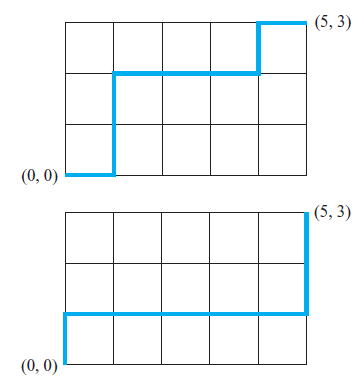
\includegraphics{images/exe33.png}
\label{fig:exe33}
\end{figure}

\begin{enumerate}[label=(\alph*)]
\item Show that each path of the type described can be represented by a bit string consisting of \emph{m} 0s and \emph{n} 1s, where a 0 represents a move one unit to the right and a 1 represents a move one unit upward.
\item Conclude from part (a) that there are $\binom{m+n}{n}$ paths of the desired type.
\end{enumerate}
%exercise 34
\item Use Exercise 33 to give an alternative proof of Corollary 2 in Section 6.3, which states that $\binom{n}{k} = \binom{n}{n-k}$ whenever \emph{k} is an integer with $0 \leq k \leq n$. [Hint: Consider the number of paths of the type described in Exercise 33 from (0, 0) to (n - k, k) and from (0, 0) to (k, n - k).]
%exercise 35
\item Use Exercise 33 to prove Theorem 4. [Hint: Count the number of paths with n steps of the type described in Exercise 33.
Every such path must end at one of the points (n - k, k) for $k = 0, 1, 2,~\cdot~\cdot~\cdot, n.]$
%exercise 36
\item Use Exercise 33 to prove Pascal’s identity. [Hint: Show that a path of the type described in Exercise 33 from (0, 0) to (n + 1 - k, k) passes through either (n + 1 - k, k - 1) or (n - k, k), but not through both.]
%exercise 37
\item Use Exercise 33 to prove the hockeystick identity from Exercise 27. [Hint: First, note that the number of paths from (0, 0) to (n + 1, r) equals $\binom{n+1+r}{r}$.
Second, count the number of paths by summing the number of these paths that start by going k units upward for $k = 0, 1, 2,~\cdot~\cdot~\cdot, r$.]
%exercise 38
\item Give a combinatorial proof that if \emph{n} is a positive integer then $\sum_{k=0}^{n}k^{2}\binom{n}{k} = n(n + 1)2^{n-2}$. [Hint: Show that both sides count the ways to select a subset of a set of \emph{n} elements together with two not necessarily distinct elements from this subset.
Furthermore, express the right-hand side as $n(n - 1)2^{n-2} + n2^{n-1}$.]
%exercise 39
\onestaritem Determine a formula involving binomial coefficients for the nth term of a sequence if its initial terms are those listed. [Hint: Looking at Pascal’s triangle will be helpful.
Although infinitely many sequences start with a specified set of terms, each of the following lists is the start of a sequence of the type desired.]
\begin{enumerate}[label=(\alph*)]
\item 1, 3, 6, 10, 15, 21, 28, 36, 45, 55, 66, . . .
\item 1, 4, 10, 20, 35, 56, 84, 120, 165, 220, . . .
\item 1, 2, 6, 20, 70, 252, 924, 3432, 12870, 48620, . . .
\item 1, 1, 2, 3, 6, 10, 20, 35, 70, 126, . . .
\item 1, 1, 1, 3, 1, 5, 15, 35, 1, 9, . . .
\item 1, 3, 15, 84, 495, 3003, 18564, 116280, 735471,4686825, . . .
\end{enumerate}
\end{enumerate}

\subsection{Generalized Permutations and Combinations}
\begin{enumerate}[label=Example~\arabic*]
%example 1
\item How many strings of length r can be formed from the uppercase letters of the English alphabet?

Solution: By the product rule, because there are 26 uppercase English letters, and because each letter can be used repeatedly, we see that there are $26^{r}$ strings of uppercase English letters of length r.

%example 2
\item How many ways are there to select four pieces of fruit from a bowl containing apples, oranges, and pears if the order in which the pieces are selected does not matter, only the type of fruit and not the individual piece matters, and there are at least four pieces of each type of fruit in the bowl?

Solution: To solve this problem we list all the ways possible to select the fruit.
There are 15 ways:

\begin{table}[h]
\centering
\begin{tabular}{ l l l }
4 apples & 4 oranges& 4 pears\\
3 apples, 1 orange & 3 apples, 1 pear & 3 oranges, 1 apple\\
3 oranges, 1 pear & 3 pears, 1 apple & 3 pears, 1 orange\\
2 apples, 2 oranges & 2 apples, 2 pears & 2 oranges, 2 pears\\
2 apples, 1 orange, 1 pear & 2 oranges, 1 apple, 1 pear & 2 pears, 1 apple, 1 orange\\
\end{tabular}
\label{tab:exe}
\end{table}
The solution is the number of \emph{4-combinations} with repetition allowed from a three-element set, \emph{{apple, orange, pear}}.

%example 3
\item How many ways are there to select five bills from a cash box containing \$1 bills, \$2 bills, \$5 bills, \$10 bills, \$20 bills, \$50 bills, and \$100 bills?
Assume that the order in which the bills are chosen does not matter, that the bills of each denomination are indistinguishable, and that there are at least five bills of each type.

Solution: Because the order in which the bills are selected does not matter and seven different types of bills can be selected as many as five times, this problem involves counting 5-combinations with repetition allowed from a set with seven elements.
Listing all possibilities would be tedious, because there are a large number of solutions.
Instead, we will illustrate the use of a technique for counting combinations with repetition allowed.
Suppose that a cash box has seven compartments, one to hold each type of bill, as illustrated in Figure~\ref{fig:bills}.
These compartments are separated by six dividers, as shown in the picture.
The choice of five bills corresponds to placing five markers in the compartments holding different types of bills.
Figure~\ref{fig:5bills} illustrates this correspondence for three different ways to select five bills, where the six dividers are represented by bars and the five bills by stars.
The number of ways to select five bills corresponds to the number of ways to arrange six bars and five stars in a row with a total of 11 positions.
Consequently, the number of ways to select the five bills is the number of ways to select the positions of the five stars from the 11 positions.
This corresponds to the number of unordered selections of 5 objects from a set of 11 objects, which can be done in C(11, 5) ways.
Consequently, there are

$C(11, 5) = \frac{11!}{5!6!} = 462$

ways to choose five bills from the cash box with seven types of bills.

\begin{figure}[h]
\centering
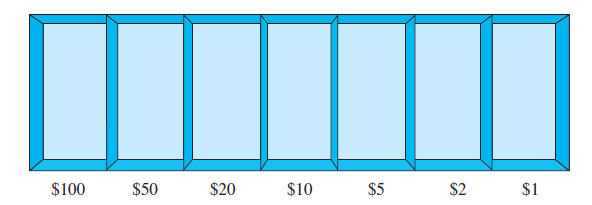
\includegraphics[height=4cm]{images/exemplo3-65.png}
\caption{\textbf{Cash Box with Seven Types of Bills.}}
\label{fig:bills}
\end{figure}

\begin{figure}[h]
\centering
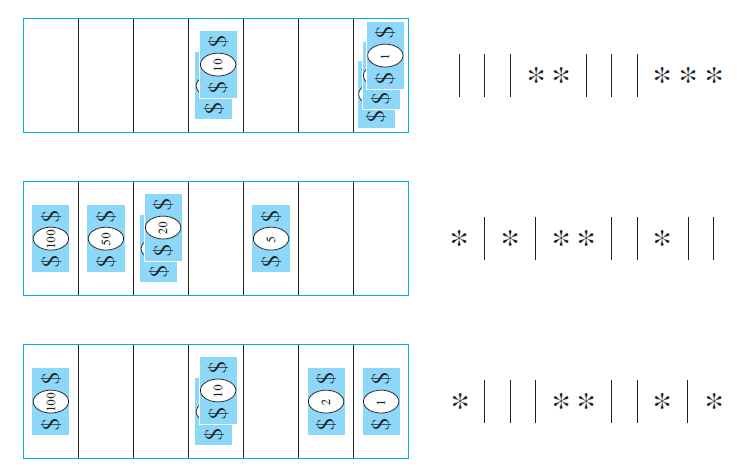
\includegraphics[height=4cm]{images/exemplo3-652.png}
\caption{\textbf{Examples of Ways to Select Five Bills.}}
\label{fig:5bills}
\end{figure}

%example 4
\item Suppose that a cookie shop has four different kinds of cookies.
How many different ways can six cookies be chosen?
Assume that only the type of cookie, and not the individual cookies or the order in which they are chosen, matters.

Solution: The number of ways to choose six cookies is the number of 6-combinations of a set
with four elements.
From Theorem 2 this equals C(4 + 6 - 1, 6) = C(9, 6).
Because

$C(9, 6) = C(9, 3) = \frac{9~\cdot8~\cdot7}{1~\cdot2~\cdot3} = 84$,

there are 84 different ways to choose the six cookies.

%example 5
\item How many solutions does the equation

$x_1 + x_2 + x_3 = 11$

have, where $x_1, x_2$, and $x_3$ are nonnegative integers?

Solution: To count the number of solutions, we note that a solution corresponds to a way of selecting 11 items from a set with three elements so that $x_1$ items of type one, $x_2$ items of type two, and $x_3$ items of type three are chosen.
Hence, the number of solutions is equal to the number of 11-combinations with repetition allowed from a set with three elements.
From Theorem 2 it follows that there are

$C(3 + 11 - 1, 11) = C(13, 11) = C(13, 2) = \frac{13 \cdot 12}{1 \cdot 2} = 78$

solutions.
The number of solutions of this equation can also be found when the variables are subject to constraints.
For instance, we can find the number of solutions where the variables are integers with $x_1 \geq 1, x_2 \geq 2$, and $x_3 \geq 3$.
A solution to the equation subject to these constraints corresponds to a selection of 11 items with $x_1$ items of type one, $x_2$ items of type two, and $x_3$ items of type three, where, in addition, there is at least one item of type one, two items of type two, and three items of type three.
So, a solution corresponds to a choice of one item of type one, two of type two, and three of type three, together with a choice of five additional items of any type.
By Theorem 2 this can be done in

$C(3 + 5 - 1, 5) = C(7, 5) = C(7, 2) = \frac{7 \cdot 6}{1 \cdot 2} = 21$

ways.
Thus, there are 21 solutions of the equation subject to the given constraints.

%example 6
\item What is the value of k after the following pseudocode has been executed?
\begin{lstlisting}[style=CStyle]
k:=0
for (*$i_1$*) := 1 to (*$n$*)
	for (*$i_2$*) := 1 to (*$i_1$*)
			.
			.
			.
		for (*$i_m$*) :=1 to (*$i_{m-1}$*)
			k := k + 1
\end{lstlisting}

Solution: Note that the initial value of k is 0 and that 1 is added to \emph{k} each time the nested loop is traversed with a sequence of integers $i_1, i_2, . . . , i_m$ such that

$1 \leq i_m \leq i_{m-1} \leq \cdot~\cdot~\cdot \leq i_1 \leq n$.

The number of such sequences of integers is the number of ways to choose \emph{m} integers from \emph{{1, 2, . . . , n}}, with repetition allowed. (To see this, note that once such a sequence has been selected, if we order the integers in the sequence in nondecreasing order, this uniquely defines an assignment of $i_m, i_{m-1}, . . . , i_1$.
Conversely, every such assignment corresponds to a unique unordered set.)
Hence, from Theorem 2, it follows that \emph{k = C(n + m - 1,m)} after this code has been executed.

%example 7
\item How many different strings can be made by reordering the letters of the word SUCCESS?

Solution: Because some of the letters of SUCCESS are the same, the answer is not given by the number of permutations of seven letters.
This word contains three Ss, two Cs, one U, and one E.
To determine the number of different strings that can be made by reordering the letters, first note that the three Ss can be placed among the seven positions in C(7, 3) different ways, leaving four positions free.
Then the two Cs can be placed in C(4, 2) ways, leaving two free positions.
The U can be placed in C(2, 1) ways, leaving just one position free.
Hence E can be placed in C(1, 1) way.
Consequently, from the product rule, the number of different strings that can be made is

$C(7, 3)C(4, 2)C(2, 1)C(1, 1) = \frac{7!}{3!4!}~\cdot~\frac{4!}{2!2!}~\cdot~\frac{2!}{1!1!}~\cdot{1!}{1!0!} = \frac{7!}{3!2!1!1!}= 420$.

%example 8
\item How many ways are there to distribute hands of 5 cards to each of four players from the standard deck of 52 cards?

Solution:We will use the product rule to solve this problem.
To begin, note that the first player can be dealt 5 cards in C(52, 5) ways.
The second player can be dealt 5 cards in C(47, 5) ways, because only 47 cards are left.
The third player can be dealt 5 cards in C(42, 5) ways.
Finally, the fourth player can be dealt 5 cards in C(37, 5) ways.
Hence, the total number of ways to deal four players 5 cards each is 

$C(52, 5)C(47, 5)C(42, 5)C(37, 5) = \frac{52!}{47!5!}~\cdot~\frac{47!}{42!5!}~\cdot~\frac{42!}{37!5!}~\cdot{37!}{32!5!} = \frac{52!}{5!5!5!5!32!}$ .

%example 9
\item How many ways are there to place 10 indistinguishable balls into eight distinguishable bins?

Solution: The number of ways to place 10 indistinguishable balls into eight bins equals the number of 10-combinations from a set with eight elements when repetition is allowed.
Consequently, there are

$C(8 + 10 - 1, 10) = C(17, 10) = \frac{17!}{10!7!} = 19,448$.

%example 10
\item How many ways are there to put four different employees into three indistinguishable offices, when each office can contain any number of employees?

Solution:We will solve this problem by enumerating all the ways these employees can be placed into the offices.
We represent the four employees by A, B, C, and D.
First, we note that we can distribute employees so that all four are put into one office, three are put into one office and a fourth is put into a second office, two employees are put into one office and two put into a second office, and finally, two are put into one office, and one each put into the other two offices.
Each way to distribute these employees to these offices can be represented by a way to partition the elements A, B, C, and D into disjoint subsets.
We can put all four employees into one office in exactly one way, represented by \{\{A,B,C,D\}\}.
We can put three employees into one office and the fourth employee into a different office in exactly four ways, represented by \{\{A,B,C\}, \{D\}\}, \{\{A,B,D\}, \{C\}\}, \{\{A,C,D\}, \{B\}\}, and \{\{B,C,D\}, \{A\}\}.
We can put two employees into one office and two into a second office in exactly three ways, represented by \{\{A,B\}, \{C,D\}\}, \{\{A,C\}, \{B,D\}\}, and \{\{A,D\}, \{B,C\}\}.
Finally, we can put two employees into one office, and one each into each of the remaining two offices in six ways, represented by \{\{A,B\}, \{C\}, \{D\}\}, \{\{A,C\}, \{B\}, \{D\}\}, \{\{A,D\}, \{B\}, \{C\}\}, \{\{B,C\}, \{A\}, \{D\}\}, \{\{B,D\}\}, \{A\}, \{C\}\}, and \{\{C,D\}, \{A\}, \{B\}\}.

Counting all the possibilities, we find that there are 14 ways to put four different employees into three indistinguishable offices.
Another way to look at this problem is to look at the number of offices into which we put employees.
Note that there are six ways to put four different employees into three indistinguishable offices so that no office is empty, seven ways to put four different employees into two indistinguishable offices so that no office is empty, and one way to put four employees into one office so that it is not empty.

%example 11
\item How many ways are there to pack six copies of the same book into four identical boxes, where a box can contain as many as six books?

Solution:We will enumerate all ways to pack the books.
For each way to pack the books, we will list the number of books in the box with the largest number of books, followed by the numbers of books in each box containing at least one book, in order of decreasing number of books in a box.
The ways we can pack the books are

6

5, 1

4, 2

4, 1, 1

3, 3

3, 2, 1

3, 1, 1, 1

2, 2, 2

2, 2, 1, 1.

For example, 4, 1, 1 indicates that one box contains four books, a second box contains a single book, and a third box contains a single book (and the fourth box is empty).
We conclude that there are nine allowable ways to pack the books, because we have listed them all.
\end{enumerate}

Exercises
\begin{enumerate}
%exercise 1
\item In how many different ways can five elements be selected in order from a set with three elements when repetition is allowed?
%exercise 2
\item In how many different ways can five elements be selected in order from a set with five elements when repetition is allowed?
%exercise 3
\item How many strings of six letters are there?
%exercise 4
\item Every day a student randomly chooses a sandwich for lunch from a pile of wrapped sandwiches.
If there are six kinds of sandwiches, how many different ways are there for the student to choose sandwiches for the seven days of a week if the order in which the sandwiches are chosen matters?
%exercise 5
\item How many ways are there to assign three jobs to five employees if each employee can be given more than one job?
%exercise 6
\item How many ways are there to select five unordered elements from a set with three elements when repetition is allowed?
%exercise 7
\item How many ways are there to select three unordered elements from a set with five elements when repetition is allowed?
%exercise 8
\item How many different ways are there to choose a dozen donuts from the 21 varieties at a donut shop?
%exercise 9
\item A bagel shop has onion bagels, poppy seed bagels, egg bagels, salty bagels, pumpernickel bagels, sesame seed bagels, raisin bagels, and plain bagels.
How many ways are there to choose
\begin{enumerate}[label=(\alph*)]
\item six bagels?
\item a dozen bagels?
\item two dozen bagels?
\item a dozen bagels with at least one of each kind?
\item a dozen bagels with at least three egg bagels and no more than two salty bagels?
\end{enumerate}
%exercise 10
\item A croissant shop has plain croissants, cherry croissants, chocolate croissants, almond croissants, apple croissants, and broccoli croissants.
How many ways are there to choose
\begin{enumerate}[label=(\alph*)]
\item a dozen croissants?
\item three dozen croissants?
\item two dozen croissants with at least two of each kind?
\item two dozen croissants with no more than two broccoli croissants?
\item two dozen croissants with at least five chocolate croissants and at least three almond croissants?
\item two dozen croissants with at least one plain croissant, at least two cherry croissants, at least three chocolate croissants, at least one almond croissant, at least two apple croissants, and no more than three broccoli croissants?
\end{enumerate}
%exercise 11
\item How many ways are there to choose eight coins from a piggy bank containing 100 identical pennies and 80 identical nickels?
%exercise 12
\item How many different combinations of pennies, nickels, dimes, quarters, and half dollars can a piggy bank contain if it has 20 coins in it?
%exercise 13
\item A book publisher has 3000 copies of a discrete mathematics book.
How many ways are there to store these books in their three warehouses if the copies of the book are indistinguishable?
%exercise 14
\item How many solutions are there to the equation 

$x_1 + x_2 + x_3 + x_4 = 17$,

where $x_1, x_2, x_3,$ and $x_4$ are nonnegative integers?
%exercise 15
\item How many solutions are there to the equation 

$x_1 + x_2 + x_3 + x_4 + x_5 = 21$,

where $x_i$ , i = 1, 2, 3, 4, 5, is a nonnegative integer such that
\begin{enumerate}[label=(\alph*)]
\item $x_1 \geq 1$?
\item $x_i \geq 2$ for i = 1, 2, 3, 4, 5?
\item $0 \leq x_1 \leq 10$?
\item $0 \leq x_1 \leq 3, 1 \leq x_2 < 4, and x3 \geq 15$?
\end{enumerate}
%exercise 16
\item How many solutions are there to the equation 

$x_1 + x_2 + x_3 + x_4 + x_5 + x_6 = 29$,

where $x_i$ , i = 1, 2, 3, 4, 5, 6, is a nonnegative integer such that
\begin{enumerate}[label=(\alph*)]
\item $x_i > 1$ for i = 1, 2, 3, 4, 5, 6?
\item $x_1 \geq 1, x_2 \geq 2, x_3 \geq 3, x_4 \geq 4, x_5 > 5$, and $x_6 \geq 6$?
\item $x_1 \geq 5$?
\item $x_1 < 8$ and $x_2 > 8$?
\end{enumerate}
%exercise 17
\item How many strings of 10 ternary digits (0, 1, or 2) are there that contain exactly two 0s, three 1s, and five 2s?
%exercise 18
\item How many strings of 20-decimal digits are there that contain two 0s, four 1s, three 2s, one 3, two 4s, three 5s, two 7s, and three 9s?
%exercise 19
\item Suppose that a large family has 14 children, including two sets of identical triplets, three sets of identical twins, and two individual children.
How many ways are there to seat these children in a row of chairs if the identical triplets or twins cannot be distinguished from one another?
%exercise 20
\item How many solutions are there to the inequality

$x_1 + x_2 + x_3 \leq 11$,

where $x_1, x_2$, and $x_3$ are nonnegative integers? [Hint: Introduce an auxiliary variable $x_4$ such that $x_1 + x_2 + x_3 + x_4 = 11$.]
%exercise 21
\item How many ways are there to distribute six indistinguishable balls into nine distinguishable bins?
%exercise 22
\item How many ways are there to distribute 12 indistinguishable balls into six distinguishable bins? 
%exercise 23
\item How many ways are there to distribute 12 distinguishable objects into six distinguishable boxes so that two objects are placed in each box?
%exercise 24
\item How many ways are there to distribute 15 distinguishable objects into five distinguishable boxes so that the boxes have one, two, three, four, and five objects in them, respectively.
%exercise 25
\item How many positive integers less than 1,000,000 have the sum of their digits equal to 19?
%exercise 26
\item How many positive integers less than 1,000,000 have exactly one digit equal to 9 and have a sum of digits equal to 13?
%exercise 27
\item There are 10 questions on a discrete mathematics final exam.
How many ways are there to assign scores to the problems if the sum of the scores is 100 and each question is worth at least 5 points?
%exercise 28
\item Show that there are $C(n + r - q_1 - q_2 -\cdot~\cdot~\cdot-q_{r-1}, n - q_1 - q_2 -\cdot~\cdot~\cdot-q_r$) different unordered selections of n objects of r different types that include at least $q_1$ objects of type one, $q_2$ objects of type two, $\cdot~\cdot~\cdot$ , and $q_r$ objects of type r.
%exercise 29
\item How many different bit strings can be transmitted if the string must begin with a 1 bit, must include three additional 1 bits (so that a total of four 1 bits is sent), must include a total of 12 0 bits, and must have at least two 0 bits following each 1 bit?
%exercise 30
\item How many different strings can be made from the letters in MISSISSIPPI, using all the letters? 
%exercise 31
\item How many different strings can be made from the letters in ABRACADABRA, using all the letters?
%exercise 32
\item How many different strings can be made from the letters in AARDVARK, using all the letters, if all three As must be consecutive?
%exercise 33
\item How many different strings can be made from the letters in ORONO, using some or all of the letters?
%exercise 34
\item How many strings with five or more characters can be formed from the letters in SEERESS?
%exercise 35
\item How many strings with seven or more characters can be formed from the letters in EVERGREEN?
%exercise 36
\item How many different bit strings can be formed using six 1s and eight 0s?
%exercise 37
\item A student has three mangos, two papayas, and two kiwi fruits.
If the student eats one piece of fruit each day, and only the type of fruit matters, in how many different ways can these fruits be consumed?
%exercise 38
\item A professor packs her collection of 40 issues of a mathematics journal in four boxes with 10 issues per box.
How many ways can she distribute the journals if
\begin{enumerate}[label=(\alph*)]
\item each box is numbered, so that they are distinguishable?
\item the boxes are identical, so that they cannot be distinguished?
\end{enumerate}
%exercise 39
\item How many ways are there to travel in \emph{xyz} space from the origin (0, 0, 0) to the point (4, 3, 5) by taking steps one unit in the positive x direction, one unit in the positive y direction, or one unit in the positive z direction? (Moving in the negative x, y, or z direction is prohibited, so that no backtracking is allowed.)
%exercise 40
\item How many ways are there to travel in \emph{xyzw} space from the origin (0, 0, 0, 0) to the point (4, 3, 5, 4) by taking steps one unit in the positive x, positive y, positive z, or positive w direction?
%exercise 41
\item How many ways are there to deal hands of seven cards to each of five players from a standard deck of 52 cards?
%exercise 42
\item In bridge, the 52 cards of a standard deck are dealt to four players.
How many different ways are there to deal bridge hands to four players?
%exercise 43
\item How many ways are there to deal hands of five cards to each of six players from a deck containing 48 different cards?
%exercise 44
\item In how many ways can a dozen books be placed on four distinguishable shelves 
\begin{enumerate}[label=(\alph*)]
\item if the books are indistinguishable copies of the same title?
\item if no two books are the same, and the positions of the books on the shelves matter? [Hint: Break this into 12 tasks, placing each book separately. Start with the sequence 1, 2, 3, 4 to represent the shelves. Represent the books by bi , i = 1, 2, . . . , 12. Place b1 to the right of one of the terms in 1, 2, 3, 4. Then successively place b2, b3, . . . , and b12.]
\end{enumerate}
%exercise 45
\item How many ways can n books be placed on k distinguishable shelves
\begin{enumerate}[label=(\alph*)]
\item if the books are indistinguishable copies of the same title?
\item if no two books are the same, and the positions of the books on the shelves matter?
\end{enumerate}
%exercise 46
\item A shelf holds 12 books in a row.
How many ways are there to choose five books so that no two adjacent books are chosen? [Hint: Represent the books that are chosen by bars and the books not chosen by stars.
Count the number of sequences of five bars and seven stars so that no two bars are adjacent.]
%exercise 47
\onestaritem Use the product rule to prove Theorem 4, by first placing objects in the first box, then placing objects in the second box, and so on.
%exercise 48
\onestaritem Prove Theorem 4 by first setting up a one-to-one correspondence between permutations of n objects with $n_i$ indistinguishable objects of type i, \emph{i =1, 2, 3, . . . , k}, and the distributions of n objects in k boxes such that $n_i$ objects are placed in box i, \emph{i = 1, 2, 3, . . . , k} and then applying Theorem 3.
%exercise 49
\onestaritem In this exercise we will prove Theorem 2 by setting up a one-to-one correspondence between the set of r-combinations with repetition allowed of \emph{S = {1, 2, 3, . . . , n}} and the set of\emph{ r-combinations} of the set \emph{T = {1, 2, 3, . . . , n + r - 1}}.
\begin{enumerate}[label=\alph*)]
\item Arrange the elements in an r-combination, with repetition allowed, of S into an increasing sequence $x_1 \leq x_2 \leq \cdot~\cdot~\cdot \leq x_r$.
Show that the sequence formed by adding \emph{k - 1} to the \emph{kth} term is strictly increasing.
Conclude that this sequence is made up of \emph{r} distinct elements from T.
\item Show that the procedure described in (a) defines a one-to-one correspondence between the set of \emph{r-combinations}, with repetition allowed, of S and the \emph{r-combinations} of T. [Hint: Show the correspondence can be reversed by associating to the \emph{r-combination} ${x_1, x_2, \cdot~\cdot~\cdot , x_r }$ of T , with $1 \leq x_1 <
x_2 < \cdot~\cdot~\cdot < x_r \leq n + r - 1$, the \emph{r-combination} with repetition allowed from S, formed by subtracting \emph{k - 1} from the \emph{kth} element.]
\item Conclude that there are C(n + r - 1, r) \emph{r-combinations} with repetition allowed from a set with \emph{n} elements.
\end{enumerate}
%exercise 50
\item How many ways are there to distribute five distinguishable objects into three indistinguishable boxes?
%exercise 51
\item How many ways are there to distribute six distinguishable objects into four indistinguishable boxes so that each of the boxes contains at least one object?
%exercise 52
\item How many ways are there to put five temporary employees into four identical offices?
%exercise 53
\item How many ways are there to put six temporary employees into four identical offices so that there is at least one temporary employee in each of these four offices?
%exercise 54
\item How many ways are there to distribute five indistinguishable objects into three indistinguishable boxes?
%exercise 55
\item How many ways are there to distribute six indistinguishable objects into four indistinguishable boxes so that each of the boxes contains at least one object?
%exercise 56
\item How many ways are there to pack eight identical DVDs into five indistinguishable boxes so that each box contains at least one DVD?
%exercise 57
\item How many ways are there to pack nine identical DVDs into three indistinguishable boxes so that each box contains at least two DVDs?
%exercise 58
\item How many ways are there to distribute five balls into seven boxes if each box must have at most one ball in it if
\begin{enumerate}[label=(\alph*)]
\item both the balls and boxes are labeled?
\item the balls are labeled, but the boxes are unlabeled?
\item the balls are unlabeled, but the boxes are labeled?
\item both the balls and boxes are unlabeled?
\end{enumerate}
%exercise 59
\item How many ways are there to distribute five balls into three boxes if each box must have at least one ball in it if
\begin{enumerate}[label=(\alph*)]
\item both the balls and boxes are labeled?
\item the balls are labeled, but the boxes are unlabeled?
\item the balls are unlabeled, but the boxes are labeled?
\item both the balls and boxes are unlabeled?
\end{enumerate}
%exercise 60
\item Suppose that a basketball league has 32 teams, split into two conferences of 16 teams each.
Each conference is split into three divisions.
Suppose that the North Central Division has five teams.
Each of the teams in the North Central Division plays four games against each of the other teams in this division, three games against each of the 11 remaining teams in the conference, and two games against each of the 16 teams in the other conference.
In how many different orders can the games of one of the teams in the North Central Division be scheduled?
%exercise 61
\onestaritem Suppose that a weapons inspector must inspect each of five different sites twice, visiting one site per day.
The inspector is free to select the order in which to visit these sites, but cannot visit site X, the most suspicious site, on two consecutive days.
In how many different orders can the inspector visit these sites?
%exercise 62
\item How many different terms are there in the expansion of $(x_1 + x_2 +\cdot~\cdot~\cdot+x_m)^{n}$ after all terms with identical sets of exponents are added?
%exercise 63
\onestaritem Prove the Multinomial Theorem: If n is a positive integer, then

$(x_1 + x_2 +\cdot~\cdot~\cdot+x_m)^{n} = \sum_{n_1+n_2 +\cdot\cdot\cdot+n_m = n} C(n; n_1, n_2,~\cdot~\cdot~\cdot, n_m)x^{n_1}_1x^{n_2}_2\cdot~\cdot~\cdot x^{nm}_m$,

where

$C(n; n_1, n_2,~\cdot~\cdot~\cdot, n_m) = \frac{n!}{n_1!n_2!~\cdot~\cdot~\cdot n_m!}$

is a \textbf{multinomial coefficient}.
%exercise 64
\item Find the expansion of $(x + y + z)^{4}$.
%exercise 65
\item Find the coefficient of $x^{3}y^{2}z^{5} in (x + y + z)^{10}$.
%exercise 66
\item How many terms are there in the expansion of 

$(x + y + z)^{100}$?
\end{enumerate}

\subsection{Generating Permutations and Combinations}
\begin{enumerate}[label=Example~\arabic*]
%example 1
\item The permutation 23415 of the set {1, 2, 3, 4, 5} precedes the permutation 23514, because these permutations agree in the first two positions, but the number in the third position in the first permutation, 4, is smaller than the number in the third position in the second permutation, 5.
Similarly, the permutation 41532 precedes 52143.

%example 2
\item What is the next permutation in lexicographic order after 362541?

Solution: The last pair of integers $a_j$ and $a_{j+1}$ where $a_j < a_{j+1}$ is $a_3 = 2$ and $a_4 = 5$.
The least integer to the right of 2 that is greater than 2 in the permutation is $a_5 = 4$.
Hence, 4 is placed in the third position.
Then the integers 2, 5, and 1 are placed in order in the last three positions, giving 125 as the last three positions of the permutation. Hence, the next permutation is 364125.

%example 3
\item Generate the permutations of the integers 1, 2, 3 in lexicographic order.

Solution: Begin with 123.
The next permutation is obtained by interchanging 3 and 2 to obtain 132.
Next, because 3 > 2 and 1 < 3, permute the three integers in 132.
Put the smaller of 3 and 2 in the first position, and then put 1 and 3 in increasing order in positions 2 and 3 to obtain 213.
This is followed by 231, obtained by interchanging 1 and 3, because 1 < 3.
The next larger permutation has 3 in the first position, followed by 1 and 2 in increasing order, namely, 312.
Finally, interchange 1 and 2 to obtain the last permutation, 321.
We have generated the permutations of 1, 2, 3 in lexicographic order.
They are 123, 132, 213, 231, 312, and 321.

%example 4
\item Find the next bit string after 10 0010 0111.

Solution: The first bit from the right that is not a 1 is the fourth bit from the right.
Change this bit to a 1 and change all the following bits to 0s.
This produces the next larger bit string, 10 0010 1000.

%example 5
\item Find the next larger 4-combination of the set {1, 2, 3, 4, 5, 6} after {1, 2, 5, 6}.

Solution: The last term among the terms $a_i$ with $a_1 = 1, a_2 = 2, a_3 = 5$, and $a_4 = 6$ such that $a_i \neq 6 - 4 + i$ is $a_2 = 2$.
To obtain the next larger 4-combination, increment $a_2$ by 1 to obtain $a+2 = 3$.
Then set $a_3 = 3 + 1 = 4$ and $a_4 = 3 + 2 = 5$.
Hence the next larger 4-combination is {1, 3, 4, 5}.
\end{enumerate}

Exercises
\begin{enumerate}
%exercise 1
\item Place these permutations of {1, 2, 3, 4, 5} in lexicographic order: 43521, 15432, 45321, 23451, 23514, 14532, 21345, 45213, 31452, 31542.
%exercise 2
\item Place these permutations of {1,2,3,4,5,6} in lexicographic order: 234561, 231456, 165432, 156423, 543216, 541236, 231465, 314562, 432561, 654321, 654312, 435612.
%exercise 3
\item The name of a file in a computer directory consists of three uppercase letters followed by a digit, where each letter is either A, B, or C, and each digit is either 1 or 2.
List the name of these files in lexicographic order, where we order letters using the usual alphabetic order of letters.
%exercise 4
\item Suppose that the name of a file in a computer directory consists of three digits followed by two lowercase letters and each digit is 0, 1, or 2, and each letter is either a or b.
List the name of these files in lexicographic order, where we order letters using the usual alphabetic order of letters.
%exercise 5
\item Find the next larger permutation in lexicographic order after each of these permutations.
\begin{enumerate}[label=(\alph*)]
\item 1432 \inlineitem 54123 \inlineitem 12453
\item 45231 \inlineitem 6714235 \inlineitem 31528764
\end{enumerate}
%exercise 6
\item Find the next larger permutation in lexicographic order after each of these permutations.
\begin{enumerate}[label=(\alph*)]
\item 1342 \inlineitem 45321 \inlineitem 13245
\item 612345 \inlineitem 1623547 \inlineitem 23587416
\end{enumerate}
%exercise 7
\item Use Algorithm 1 to generate the 24 permutations of the first four positive integers in lexicographic order.
%exercise 8
\item Use Algorithm 2 to list all the subsets of the set {1, 2, 3, 4}.
%exercise 9
\item Use Algorithm 3 to list all the 3-combinations of {1, 2, 3, 4, 5}.
%exercise 10
\item Show that Algorithm 1 produces the next larger permutation in lexicographic order.
%exercise 11
\item Show that Algorithm 3 produces the next larger r-combination in lexicographic order after a given r-combination.
%exercise 12
\item Develop an algorithm for generating the r-permutations of a set of n elements.
%exercise 13
\item List all 3-permutations of {1, 2, 3, 4, 5}.

The remaining exercises in this section develop another algorithm for generating the permutations of {1, 2, 3, . . . , n}.
This algorithm is based on Cantor expansions of integers.
Every nonnegative integer less than n! has a unique Cantor expansion

$a_11! + a_22!+~\cdot~\cdot~\cdot+a)n-1(n - 1)!$

where $a_i$ is a nonnegative integer not exceeding i, for $i = 1, 2,~\cdot~\cdot~\cdot, n - 1$.
The integers $a_1, a_2,~\cdot~\cdot~\cdot, a_{n-1}$ are called the \textbf{Cantor digits} of this integer.

Given a permutation of ${1, 2,~\cdot~\cdot~\cdot, n}$, let $a_{k-1}, k = 2, 3,~\cdot~\cdot~\cdot, n$, be the number of integers less than k that follow k in the permutation.
For instance, in the permutation 43215, $a_1$ is the number of integers less than 2 that follow 2, so $a_1 = 1$.
Similarly, for this example $a_2 = 2, a_3 = 3$, and $a_4 = 0$.
Consider the function from the set of permutations of ${1, 2, 3,~\cdot~\cdot~\cdot, n}$ to the set of nonnegative integers less than n! that sends a permutation to the integer that has $a_1, a_2,~\cdot~\cdot~\cdot, a_{n-1}$, defined in this way, as its Cantor digits.
%exercise 14
\item Find the Cantor digits $a_1, a_2~\cdot~\cdot~\cdot, a_{n-1}$ that correspond to these permutations.
\begin{enumerate}[label=(\alph*)]
\item 246531 \inlineitem 12345 \inlineitem 654321
\end{enumerate}
%exercise 15
\onestaritem Show that the correspondence described in the preamble is a bijection between the set of permutations of {1, 2, 3, . . . , n} and the nonnegative integers less than n!.
%exercise 16
\item Find the permutations of {1, 2, 3, 4, 5} that correspond to these integers with respect to the correspondence between Cantor expansions and permutations as described in the preamble to Exercise 14.
\begin{enumerate}[label=(\alph*)]
\item 3 \inlineitem 89 \inlineitem 111
\end{enumerate}
%exercise 17
\item Develop an algorithm for producing all permutations of a set of n elements based on the correspondence described in the preamble to Exercise 14.
\end{enumerate}
\end{document}